% ==========================================
% BAB III ANALISIS DAN PERANCANGAN ARSITEKTUR REFERENSI PERTAHANAN
% ==========================================
\cleardoublepage
\chapter{ANALISIS DAN PERANCANGAN ARSITEKTUR REFERENSI PERTAHANAN}
\label{chap:III}

\section{Analisis Kebutuhan Arsitektur Referensi}
\label{sec:III.1}

Analisis kebutuhan merumuskan kebutuhan yang harus dipenuhi oleh arsitektur referensi pertahanan. Analisis ini merupakan pelaksanaan tahap \textit{Defining the Objectives for a Solution} pada DSRM \cite{Peffers2007}. Alur analisis ditunjukkan pada Gambar~\ref{fig:III.1}.

\begin{figure}[htbp]
\centering
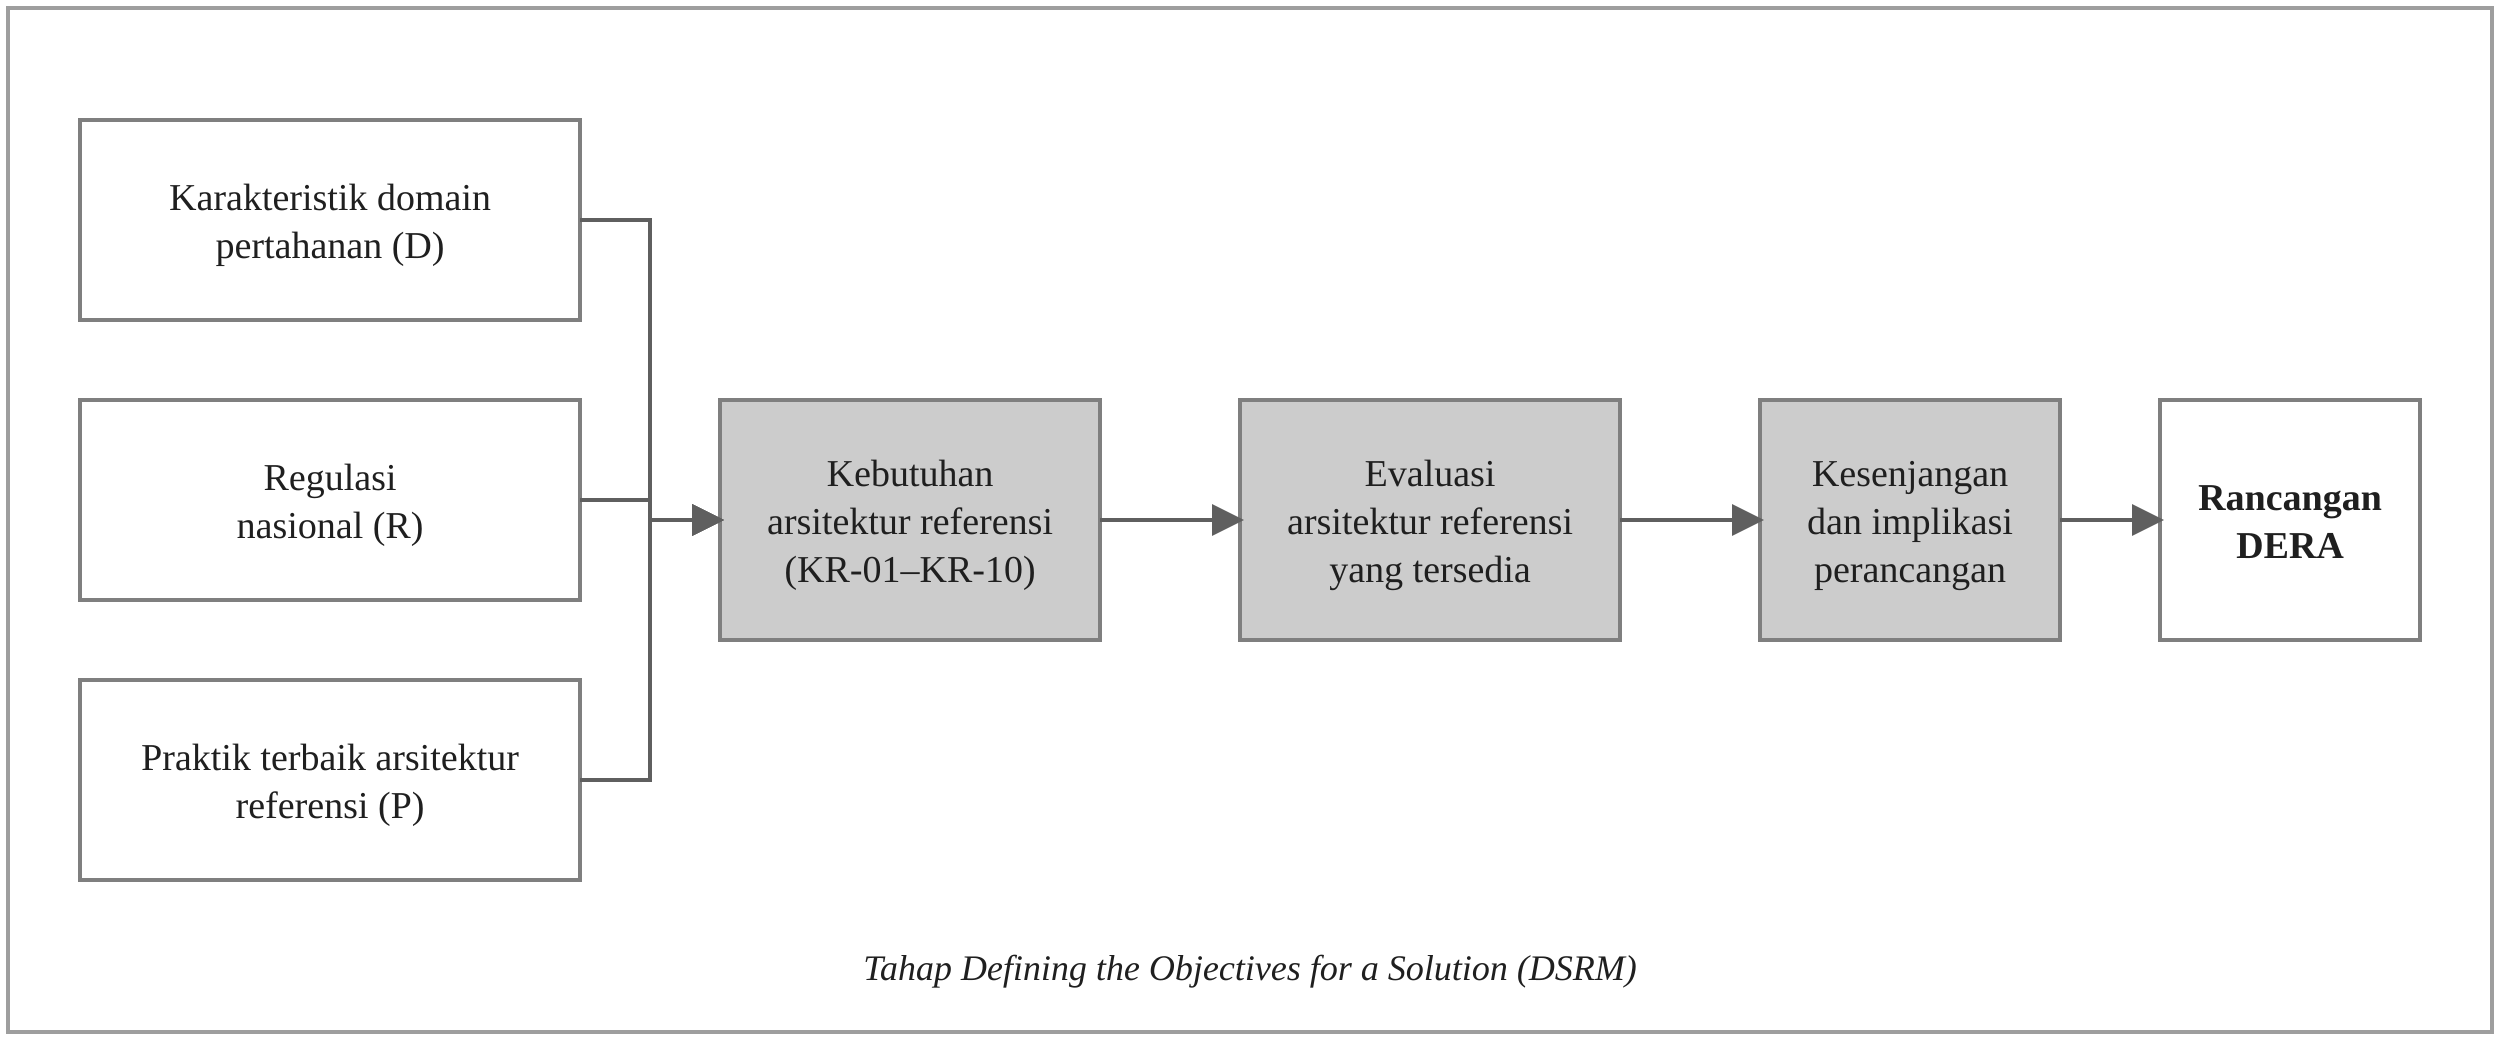
\includegraphics[width=1.00\linewidth,height=0.8\textheight,keepaspectratio]{images/Alur Analisis Kebutuhan Arsitektur Referensi.png}
\caption{Alur Analisis Kebutuhan Arsitektur Referensi}
\label{fig:III.1}
\end{figure}

Gambar~\ref{fig:III.1} menunjukkan bahwa kebutuhan arsitektur referensi dirumuskan dari tiga sumber, kemudian digunakan untuk mengevaluasi arsitektur referensi yang tersedia. Kebutuhan yang belum terpenuhi menjadi kesenjangan, dan kesenjangan tersebut diterjemahkan menjadi implikasi perancangan \textit{Defense Enterprise Reference Architecture} (DERA).

\subsection{Sumber dan Metode Perumusan Kebutuhan}
\label{sec:III.1.1}

Kebutuhan arsitektur referensi dirumuskan secara deduktif dari tiga sumber berikut.

\begin{enumerate}[label=\arabic*.]
\item Karakteristik domain pertahanan (D), berdasarkan kajian transformasi digital pertahanan, NCW, JADC2, dan C6ISR pada Bab II.
\item Regulasi nasional (R), yaitu kewajiban SPBE dan Arsitektur SPBE Nasional \cite{Perpres95Tahun2018,Perpres132Tahun2022}, percepatan transformasi digital \cite{Perpres82Tahun2023}, Satu Data Pertahanan \cite{Permenhan1Tahun2023}, Pedoman Pertahanan Siber \cite{Permenhan82Tahun2014}, serta peta jalan pelindungan infrastruktur informasi vital sektor pertahanan \cite{Permenhan34Tahun2025}.
\item Praktik terbaik arsitektur referensi (P), yaitu komponen arsitektur referensi \cite{DoDCIO2010RA}, karakteristik dan metode perancangannya \cite{Cloutier2010,Angelov2012,Galster2011}, kedudukannya dalam TOGAF \cite{TOGAF2022}, serta contoh arsitektur referensi sektoral \cite{UNECECSPA2014}.
\end{enumerate}

Ketiga sumber tersebut disintesiskan menjadi sepuluh kebutuhan arsitektur referensi dengan kode KR-01 hingga KR-10.

\subsection{Karakteristik Domain Pertahanan}
\label{sec:III.1.2}

Karakteristik domain pertahanan yang membedakannya dari domain pemerintahan umum dirangkum pada Tabel~\ref{tab:III.1}.

\begingroup\small\setstretch{1.0}
\begin{longtable}{@{}>{\raggedright\arraybackslash\hspace{0pt}}p{0.057\linewidth}>{\raggedright\arraybackslash\hspace{0pt}}p{0.194\linewidth}>{\raggedright\arraybackslash\hspace{0pt}}p{0.370\linewidth}>{\raggedright\arraybackslash\hspace{0pt}}p{0.286\linewidth}@{}}
\caption{Karakteristik Domain Pertahanan}\label{tab:III.1}\\
\toprule
\textbf{No.} & \textbf{Karakteristik} & \textbf{Uraian} & \textbf{Implikasi bagi Arsitektur Referensi}\\
\midrule
\endfirsthead
\multicolumn{4}{@{}l}{\small\itshape \tablename\ \thetable{} (lanjutan)}\\
\toprule
\textbf{No.} & \textbf{Karakteristik} & \textbf{Uraian} & \textbf{Implikasi bagi Arsitektur Referensi}\\
\midrule
\endhead
\bottomrule
\endlastfoot
\centering\arraybackslash 1 & Banyak entitas dengan kewenangan berbeda & Kemhan RI menetapkan kebijakan dan standar, Mabes TNI mengendalikan operasi, ketiga matra melaksanakan misi, dan industri pertahanan menyediakan alutsista \cite{UU3Tahun2025,Permenhan8Tahun2016}. & Acuan bersama lintas organisasi dengan pembagian kewenangan yang jelas.\\*
\centering\arraybackslash 2 & Siklus operasi terpadu & Efektivitas operasi bergantung pada keterpaduan ISR, komando-kendali, dan unsur penindak \cite{USDoD2022}. & Keterpaduan kapabilitas lintas domain arsitektur.\\
\centering\arraybackslash 3 & Informasi terklasifikasi dan ancaman siber & Data pertahanan diklasifikasikan Terbuka, Terbatas, dan Rahasia \cite{Permenhan1Tahun2023}, sedangkan ancaman siber menyasar perangkat dan data pertahanan \cite{Permenhan82Tahun2014}. & Keamanan sejak perancangan dan pemisahan domain klasifikasi.\\
\centering\arraybackslash 4 & Ketergantungan pada jaringan dan waktu nyata & NCW dan JADC2 menuntut pertukaran data yang cepat dan andal lintas domain operasi \cite{Koch2015,USDoD2022}. & Interoperabilitas, ketersediaan, dan ketahanan komunikasi.\\
\centering\arraybackslash 5 & Sistem dan alutsista yang heterogen & Komando dan kendali serta sistem tempur dikembangkan per matra dengan standar yang berbeda (Tabel~\ref{tab:II.1}). & Standar antarmuka dan \textit{building blocks} bersama.\\*
\centering\arraybackslash 6 & Peran ganda administratif dan operasional & Kemhan RI wajib menyusun Arsitektur SPBE sekaligus mendukung kapabilitas operasional pertahanan \cite{Perpres95Tahun2018,Perpres132Tahun2022}. & Keselarasan dengan Arsitektur SPBE tanpa kehilangan muatan operasional.\\
\end{longtable}
\endgroup

Tabel~\ref{tab:III.1} menunjukkan bahwa arsitektur referensi pertahanan harus berlaku lintas organisasi, menjaga keterpaduan siklus operasi, melindungi informasi terklasifikasi, dan tetap selaras dengan kewajiban pemerintahan.

\subsection{Identifikasi Kebutuhan Arsitektur Referensi}
\label{sec:III.1.3}

Hasil sintesis berupa sepuluh kebutuhan arsitektur referensi disajikan pada Tabel~\ref{tab:III.2}.

\begingroup\small\setstretch{1.0}
\begin{longtable}{@{}>{\raggedright\arraybackslash\hspace{0pt}}p{0.103\linewidth}>{\raggedright\arraybackslash\hspace{0pt}}p{0.252\linewidth}>{\raggedright\arraybackslash\hspace{0pt}}p{0.415\linewidth}>{\raggedright\arraybackslash\hspace{0pt}}p{0.137\linewidth}@{}}
\caption{Kebutuhan Arsitektur Referensi Pertahanan}\label{tab:III.2}\\
\toprule
\textbf{Kode} & \textbf{Kebutuhan} & \textbf{Deskripsi} & \textbf{Sumber}\\
\midrule
\endfirsthead
\multicolumn{4}{@{}l}{\small\itshape \tablename\ \thetable{} (lanjutan)}\\
\toprule
\textbf{Kode} & \textbf{Kebutuhan} & \textbf{Deskripsi} & \textbf{Sumber}\\
\midrule
\endhead
\bottomrule
\endlastfoot
KR-01 & Keterpaduan kapabilitas C6ISR & Memodelkan kapabilitas kesembilan unsur C6ISR beserta keterpaduan siklus ISR, komando-kendali, dan unsur penindak. & \centering\arraybackslash D\\*
KR-02 & Cakupan empat domain arsitektur & Menyediakan acuan domain bisnis, data, aplikasi, dan teknologi yang saling terhubung. & \centering\arraybackslash P, R\\
KR-03 & Keamanan sejak perancangan & Menanamkan keamanan siber dan klasifikasi informasi sejak tahap perancangan. & \centering\arraybackslash D, R\\
KR-04 & Interoperabilitas lintas entitas & Mendukung pertukaran data antara Kemhan RI, Mabes TNI, ketiga matra, dan industri pertahanan. & \centering\arraybackslash D, R\\
KR-05 & Keterkaitan dengan doktrin dan strategi pertahanan & Menautkan komponen arsitektur dengan doktrin dan sasaran strategis pertahanan. & \centering\arraybackslash D\\
KR-06 & Keselarasan dengan regulasi nasional & Selaras dengan Arsitektur SPBE, Satu Data Pertahanan, dan kebijakan pertahanan siber. & \centering\arraybackslash R\\
KR-07 & Kelengkapan komponen arsitektur referensi & Memuat tujuan strategis, prinsip, posisi teknis, pola, dan kosakata. & \centering\arraybackslash P\\
KR-08 & Keterlacakan & Setiap komponen dapat ditelusuri ke kebutuhan dan unsur C6ISR. & \centering\arraybackslash P\\
KR-09 & Dapat digunakan ulang dan disesuaikan & Bersifat generik bagi organisasi pertahanan dan menyediakan titik variasi untuk penyesuaian. & \centering\arraybackslash P\\*
KR-10 & Dapat diterapkan dengan metode EA baku & Menyediakan panduan penerapan dalam TOGAF ADM dan kriteria kesesuaian arsitektur. & \centering\arraybackslash P\\
\end{longtable}
\endgroup

Keterangan: D = domain pertahanan; R = regulasi nasional; P = praktik terbaik arsitektur referensi. Tabel~\ref{tab:III.2} menunjukkan bahwa kebutuhan terbagi dalam empat kelompok, yaitu muatan pertahanan (KR-01, KR-03, KR-04, dan KR-05), keselarasan nasional (KR-06), kualitas arsitektur referensi (KR-02, KR-07, KR-08, dan KR-09), serta penerapan (KR-10). Kelompok kualitas menjadi dasar kriteria evaluasi pada Bab V, yaitu \textit{completeness} (KR-01, KR-02, dan KR-07), \textit{consistency} (KR-02), \textit{traceability} (KR-08), serta \textit{reusability} dan \textit{adaptability} (KR-09).

\subsection{Evaluasi Pemenuhan Kebutuhan oleh Arsitektur Referensi yang Ada}
\label{sec:III.1.4}

Kesepuluh kebutuhan tersebut digunakan untuk mengevaluasi empat acuan yang dibahas pada Bab II, yaitu NATO C3 \textit{Taxonomy} \cite{NATOC3Taxonomy}, arsitektur referensi C2 DSTA \cite{Chang2009}, Referensi Arsitektur SPBE Nasional \cite{Perpres132Tahun2022}, dan model referensi TOGAF \cite{TOGAF2022}. Penilaian menggunakan tiga tingkat pemenuhan, yaitu terpenuhi (T), terpenuhi sebagian (TS), dan tidak terpenuhi (TT). Hasil evaluasi disajikan pada Tabel~\ref{tab:III.3}.

\begingroup\small\setstretch{1.0}
\begin{longtable}{@{}>{\raggedright\arraybackslash\hspace{0pt}}p{0.280\linewidth}>{\raggedright\arraybackslash\hspace{0pt}}p{0.149\linewidth}>{\raggedright\arraybackslash\hspace{0pt}}p{0.149\linewidth}>{\raggedright\arraybackslash\hspace{0pt}}p{0.149\linewidth}>{\raggedright\arraybackslash\hspace{0pt}}p{0.149\linewidth}@{}}
\caption{Evaluasi Pemenuhan Kebutuhan oleh Arsitektur Referensi yang Ada}\label{tab:III.3}\\
\toprule
\textbf{Kebutuhan} & \textbf{NATO C3 \textit{Taxonomy}} & \textbf{Arsitektur Referensi C2 DSTA} & \textbf{Referensi Arsitektur SPBE Nasional} & \textbf{Model Referensi TOGAF}\\
\midrule
\endfirsthead
\multicolumn{5}{@{}l}{\small\itshape \tablename\ \thetable{} (lanjutan)}\\
\toprule
\textbf{Kebutuhan} & \textbf{NATO C3 \textit{Taxonomy}} & \textbf{Arsitektur Referensi C2 DSTA} & \textbf{Referensi Arsitektur SPBE Nasional} & \textbf{Model Referensi TOGAF}\\
\midrule
\endhead
\bottomrule
\endlastfoot
KR-01 Keterpaduan kapabilitas C6ISR & \centering\arraybackslash TS & \centering\arraybackslash TS & \centering\arraybackslash TT & \centering\arraybackslash TT\\*
KR-02 Cakupan empat domain & \centering\arraybackslash TS & \centering\arraybackslash TS & \centering\arraybackslash T & \centering\arraybackslash TS\\
KR-03 Keamanan sejak perancangan & \centering\arraybackslash TS & \centering\arraybackslash TS & \centering\arraybackslash TS & \centering\arraybackslash TS\\
KR-04 Interoperabilitas lintas entitas & \centering\arraybackslash T & \centering\arraybackslash T & \centering\arraybackslash TS & \centering\arraybackslash TS\\
KR-05 Doktrin dan strategi pertahanan & \centering\arraybackslash TS & \centering\arraybackslash TT & \centering\arraybackslash TT & \centering\arraybackslash TT\\
KR-06 Keselarasan dengan regulasi nasional & \centering\arraybackslash TT & \centering\arraybackslash TT & \centering\arraybackslash T & \centering\arraybackslash TS\\
KR-07 Kelengkapan komponen & \centering\arraybackslash TS & \centering\arraybackslash TS & \centering\arraybackslash TS & \centering\arraybackslash TS\\
KR-08 Keterlacakan & \centering\arraybackslash TS & \centering\arraybackslash TT & \centering\arraybackslash TS & \centering\arraybackslash TS\\
KR-09 Dapat digunakan ulang dan disesuaikan & \centering\arraybackslash T & \centering\arraybackslash T & \centering\arraybackslash T & \centering\arraybackslash T\\*
KR-10 Dapat diterapkan dengan metode EA baku & \centering\arraybackslash TS & \centering\arraybackslash TT & \centering\arraybackslash TS & \centering\arraybackslash T\\
\end{longtable}
\endgroup

Keterangan: T = terpenuhi; TS = terpenuhi sebagian; TT = tidak terpenuhi. Tabel~\ref{tab:III.3} menunjukkan bahwa NATO C3 \textit{Taxonomy} dan arsitektur referensi C2 DSTA kuat dalam interoperabilitas dan muatan komando-kendali, tetapi belum mencakup seluruh unsur C6ISR dan disusun untuk konteks NATO dan Singapura. Referensi Arsitektur SPBE Nasional kuat dalam keselarasan nasional dan cakupan domain, tetapi tidak memuat muatan pertahanan. Model referensi TOGAF mudah diterapkan melalui ADM, tetapi bersifat generik. Tidak satu pun acuan memenuhi KR-01 dan KR-05 secara penuh, dan hanya Referensi Arsitektur SPBE Nasional yang memenuhi KR-06.

\subsection{Implikasi terhadap Perancangan}
\label{sec:III.1.5}

Hasil evaluasi menunjukkan bahwa kebutuhan arsitektur referensi pertahanan Indonesia tidak dapat dipenuhi dengan mengadopsi salah satu acuan yang ada. Oleh karena itu, dibutuhkan arsitektur referensi baru yang memadukan muatan pertahanan, keselarasan nasional, dan kemudahan penerapan. Implikasi setiap kebutuhan terhadap perancangan DERA disajikan pada Tabel~\ref{tab:III.4}.

\begingroup\small\setstretch{1.0}
\begin{longtable}{@{}>{\raggedright\arraybackslash\hspace{0pt}}p{0.106\linewidth}>{\raggedright\arraybackslash\hspace{0pt}}p{0.390\linewidth}>{\raggedright\arraybackslash\hspace{0pt}}p{0.441\linewidth}@{}}
\caption{Implikasi Kebutuhan terhadap Perancangan DERA}\label{tab:III.4}\\
\toprule
\textbf{Kode} & \textbf{Kesenjangan Utama} & \textbf{Implikasi Perancangan}\\
\midrule
\endfirsthead
\multicolumn{3}{@{}l}{\small\itshape \tablename\ \thetable{} (lanjutan)}\\
\toprule
\textbf{Kode} & \textbf{Kesenjangan Utama} & \textbf{Implikasi Perancangan}\\
\midrule
\endhead
\bottomrule
\endlastfoot
KR-01 & Belum ada model kapabilitas yang memadukan sembilan unsur C6ISR. & \textit{Capability Reference Model} berbasis C6ISR dan pola lintas domain C6ISR.\\*
KR-02 & Acuan pertahanan tidak mencakup empat domain secara terhubung. & Arsitektur referensi empat domain yang dihubungkan oleh metamodel DERA.\\
KR-03 & Keamanan belum mengikat dan klasifikasi pertahanan belum dimodelkan. & Prinsip \textit{Security by Design}, posisi teknis klasifikasi data, dan pola pemisahan domain klasifikasi.\\
KR-04 & Interoperabilitas belum diarahkan pada entitas pertahanan Indonesia. & Prinsip \textit{Interoperability} serta standar dan \textit{building blocks} interoperabilitas.\\
KR-05 & Belum ada penautan dengan doktrin dan strategi pertahanan Indonesia. & Tujuan strategis DERA serta penautan prinsip dengan doktrin dan strategi pertahanan.\\
KR-06 & Acuan pertahanan belum selaras dengan regulasi nasional. & Pemetaan DERA ke domain Arsitektur SPBE dan posisi teknis berbasis regulasi.\\
KR-07 & Komponen arsitektur referensi belum lengkap. & Struktur DERA mengikuti lima komponen arsitektur referensi.\\
KR-08 & Keterlacakan belum dinyatakan secara eksplisit. & Metamodel DERA dan matriks keterlacakan.\\
KR-09 & Telah terpenuhi pada acuan lain dan harus dipertahankan. & Titik variasi serta mekanisme adopsi dan penyesuaian.\\*
KR-10 & Acuan pertahanan belum memiliki panduan penerapan dalam ADM. & Panduan pemanfaatan DERA pada fase ADM dan kriteria kesesuaian arsitektur.\\
\end{longtable}
\endgroup

Tabel~\ref{tab:III.4} menunjukkan bahwa setiap kebutuhan memiliki implikasi yang dapat ditelusuri ke komponen DERA. Implikasi tersebut menjadi spesifikasi rancangan DERA pada subbab berikutnya.

\section{Pendekatan Perancangan}
\label{sec:III.2}

Subbab ini menguraikan strategi perancangan DERA, sintesis sumber rancangan, pemetaan unsur C6ISR terhadap domain arsitektur, serta struktur dan metamodel DERA.

\subsection{Strategi Perancangan}
\label{sec:III.2.1}

DERA dirancang dengan mengadaptasi enam langkah perancangan arsitektur referensi menurut \textcite{Galster2011}. Penerapan setiap langkah dalam penelitian ini disajikan pada Tabel~\ref{tab:III.5}.

\begingroup\small\setstretch{1.0}
\begin{longtable}{@{}>{\raggedright\arraybackslash\hspace{0pt}}p{0.272\linewidth}>{\raggedright\arraybackslash\hspace{0pt}}p{0.524\linewidth}>{\raggedright\arraybackslash\hspace{0pt}}p{0.142\linewidth}@{}}
\caption{Langkah Perancangan DERA}\label{tab:III.5}\\
\toprule
\textbf{Langkah} & \textbf{Penerapan dalam Penelitian Ini} & \textbf{Lokasi}\\
\midrule
\endfirsthead
\multicolumn{3}{@{}l}{\small\itshape \tablename\ \thetable{} (lanjutan)}\\
\toprule
\textbf{Langkah} & \textbf{Penerapan dalam Penelitian Ini} & \textbf{Lokasi}\\
\midrule
\endhead
\bottomrule
\endlastfoot
1. Menentukan jenis arsitektur referensi & DERA ditetapkan sebagai arsitektur referensi sektoral tingkat \textit{enterprise} (\textit{Industry Architecture}) untuk menstandarkan dan memfasilitasi interoperabilitas antarorganisasi pertahanan. & III.2.1\\*
2. Memilih strategi perancangan & DERA dirancang dari awal dengan menyintesis konsep dan praktik yang ada, bukan dari arsitektur yang telah berjalan. & III.2.2\\
3. Menghimpun data empiris & Literatur, regulasi, dokumen Kemhan RI, serta hasil wawancara dengan unit kerja Kemhan RI. & III.1\\
4. Menyusun arsitektur referensi & Fondasi dan model referensi DERA. & III.3–III.4\\
5. Menambahkan variabilitas & Mekanisme adopsi dan penyesuaian. & III.5\\*
6. Mengevaluasi arsitektur referensi & Demonstrasi pada Kemhan RI serta evaluasi lima kriteria. & Bab IV–V\\
\end{longtable}
\endgroup

Tabel~\ref{tab:III.5} menunjukkan bahwa DERA dirancang dari awal. Untuk arsitektur referensi yang dirancang dari awal, Galster dan Avgeriou menyarankan evaluasi melalui penerapan bertahap dan daftar periksa \cite{Galster2011}. Saran tersebut sejalan dengan demonstrasi pada Kemhan RI dan evaluasi analitis pada Bab V.

\subsection{Sintesis C6ISR, Framework Pertahanan, TOGAF, dan Regulasi Nasional}
\label{sec:III.2.2}

DERA disusun dengan menyintesis beberapa sumber yang masing-masing memberikan kontribusi berbeda, sebagaimana disajikan pada Tabel~\ref{tab:III.6}.

\begingroup\small\setstretch{1.0}
\begin{longtable}{@{}>{\raggedright\arraybackslash\hspace{0pt}}p{0.318\linewidth}>{\raggedright\arraybackslash\hspace{0pt}}p{0.651\linewidth}@{}}
\caption{Sumber dan Kontribusi bagi DERA}\label{tab:III.6}\\
\toprule
\textbf{Sumber} & \textbf{Kontribusi bagi DERA}\\
\midrule
\endfirsthead
\multicolumn{2}{@{}l}{\small\itshape \tablename\ \thetable{} (lanjutan)}\\
\toprule
\textbf{Sumber} & \textbf{Kontribusi bagi DERA}\\
\midrule
\endhead
\bottomrule
\endlastfoot
C6ISR \cite{Petrovski2023,Todorovic2025} & Unsur kapabilitas dan siklus ISR, komando-kendali, dan unsur penindak sebagai muatan \textit{Capability Reference Model}.\\*
DoDAF, NAF, MODAF, dan UAF \cite{DoDAF2010v202,NAFv41,MODAF2012,OMGUAF2022} & \textit{Viewpoint} kapabilitas dan operasional serta konsep meta-model pertahanan.\\
NATO C3 \textit{Taxonomy} \cite{NATOC3Taxonomy} & Pola taksonomi kapabilitas dan layanan sebagai acuan struktur model kapabilitas.\\
TOGAF \cite{TOGAF2022} & Empat domain arsitektur, \textit{building blocks}, \textit{enterprise metamodel}, \textit{Enterprise Continuum}, dan ADM.\\
\textit{DoD Reference Architecture Description} \cite{DoDCIO2010RA} & Lima komponen arsitektur referensi.\\
CSPA \cite{UNECECSPA2014} & Struktur arsitektur referensi sektoral, yaitu prinsip berkategori, perspektif arsitektur, dan komponen yang dapat digunakan ulang.\\*
Regulasi nasional \cite{Perpres95Tahun2018,Permenhan1Tahun2023,Permenhan82Tahun2014,Perpres132Tahun2022} & Posisi teknis dan keselarasan dengan SPBE, Satu Data Pertahanan, klasifikasi informasi, dan keamanan siber.\\
\end{longtable}
\endgroup

Tabel~\ref{tab:III.6} menunjukkan bahwa C6ISR berperan sebagai sumber muatan, TOGAF sebagai struktur dan metode, \textit{framework} pertahanan dan NATO C3 \textit{Taxonomy} sebagai rujukan pola, serta regulasi nasional sebagai batasan rancangan.

\subsection{Pemetaan Unsur C6ISR terhadap Domain Arsitektur}
\label{sec:III.2.3}

Pemetaan dilakukan untuk menentukan cara setiap unsur C6ISR diterjemahkan ke dalam empat domain arsitektur. Unsur C6ISR dikelompokkan menjadi enam kelompok, yaitu \textit{command \& control}, ISR, \textit{combat systems}, \textit{communications}, \textit{computers}, dan \textit{cyber-defense}. Hasil pemetaan disajikan pada Tabel~\ref{tab:III.7}.

\begingroup\small\setstretch{1.0}
\begin{longtable}{@{}>{\raggedright\arraybackslash\hspace{0pt}}p{0.155\linewidth}>{\raggedright\arraybackslash\hspace{0pt}}p{0.180\linewidth}>{\raggedright\arraybackslash\hspace{0pt}}p{0.180\linewidth}>{\raggedright\arraybackslash\hspace{0pt}}p{0.180\linewidth}>{\raggedright\arraybackslash\hspace{0pt}}p{0.180\linewidth}@{}}
\caption{Pemetaan Unsur C6ISR terhadap Domain Arsitektur}\label{tab:III.7}\\
\toprule
\textbf{Unsur C6ISR} & \textbf{Bisnis} & \textbf{Data} & \textbf{Aplikasi} & \textbf{Teknologi}\\
\midrule
\endfirsthead
\multicolumn{5}{@{}l}{\small\itshape \tablename\ \thetable{} (lanjutan)}\\
\toprule
\textbf{Unsur C6ISR} & \textbf{Bisnis} & \textbf{Data} & \textbf{Aplikasi} & \textbf{Teknologi}\\
\midrule
\endhead
\bottomrule
\endlastfoot
\textit{Command \& Control} & Kewenangan komando berjenjang serta proses perencanaan dan pengendalian operasi & Data situasi operasional dan rencana operasi & Aplikasi komando-kendali dan tampilan pemantauan terpusat & Infrastruktur pusat komando\\*
ISR & Proses pengumpulan dan analisis intelijen & Data sensor dan intelijen terklasifikasi & Aplikasi fusi data dan kesadaran situasi & Antarmuka sensor dan platform ISR\\
\textit{Combat Systems} & Kebijakan dan persyaratan pengadaan alutsista yang interoperabel & Data status kekuatan dan hasil penindakan & Antarmuka komando-kendali dengan sistem tempur & Standar antarmuka alutsista\\
\textit{Communications} & Kebijakan komunikasi strategis & Format pertukaran data dan pesan & Layanan pertukaran pesan & Jaringan, satelit, dan jalur komunikasi cadangan\\
\textit{Computers} & Tata kelola layanan TIK dan data & Tata kelola dan fusi data & Analitik dan dukungan keputusan & Pusat data, pemulihan bencana, dan komputasi \textit{edge}\\*
\textit{Cyber-Defense} & Kebijakan dan organisasi pertahanan siber & Klasifikasi dan pelindungan data & Keamanan aplikasi dan manajemen identitas & Pemisahan jaringan terklasifikasi dan pusat operasi keamanan\\
\end{longtable}
\endgroup

Tabel~\ref{tab:III.7} menunjukkan bahwa pada tingkat EA, setiap unsur C6ISR memiliki padanan pada keempat domain arsitektur. \textit{Combat systems} diterjemahkan melalui kebijakan pengadaan, data status kekuatan, antarmuka, dan standar antarmuka alutsista, bukan melalui desain teknis operasi tempur, sesuai dengan ruang lingkup penelitian. Namun, pemetaan per domain berisiko memecah keterpaduan C6ISR sebagaimana dibahas pada II.7.3. Oleh karena itu, DERA menggunakan dua elemen pengikat, yaitu \textit{Capability Reference Model} yang menjaga siklus ISR, komando-kendali, dan unsur penindak sebagai rantai kapabilitas, serta pola lintas domain yang memadukan elemen keempat domain untuk setiap fungsi C6ISR.

\subsection{Struktur dan Metamodel DERA}
\label{sec:III.2.4}

Berdasarkan implikasi perancangan pada Tabel~\ref{tab:III.4}, DERA disusun dalam tiga lapis, sebagaimana ditunjukkan pada Gambar~\ref{fig:III.2}.

\begin{figure}[htbp]
\centering
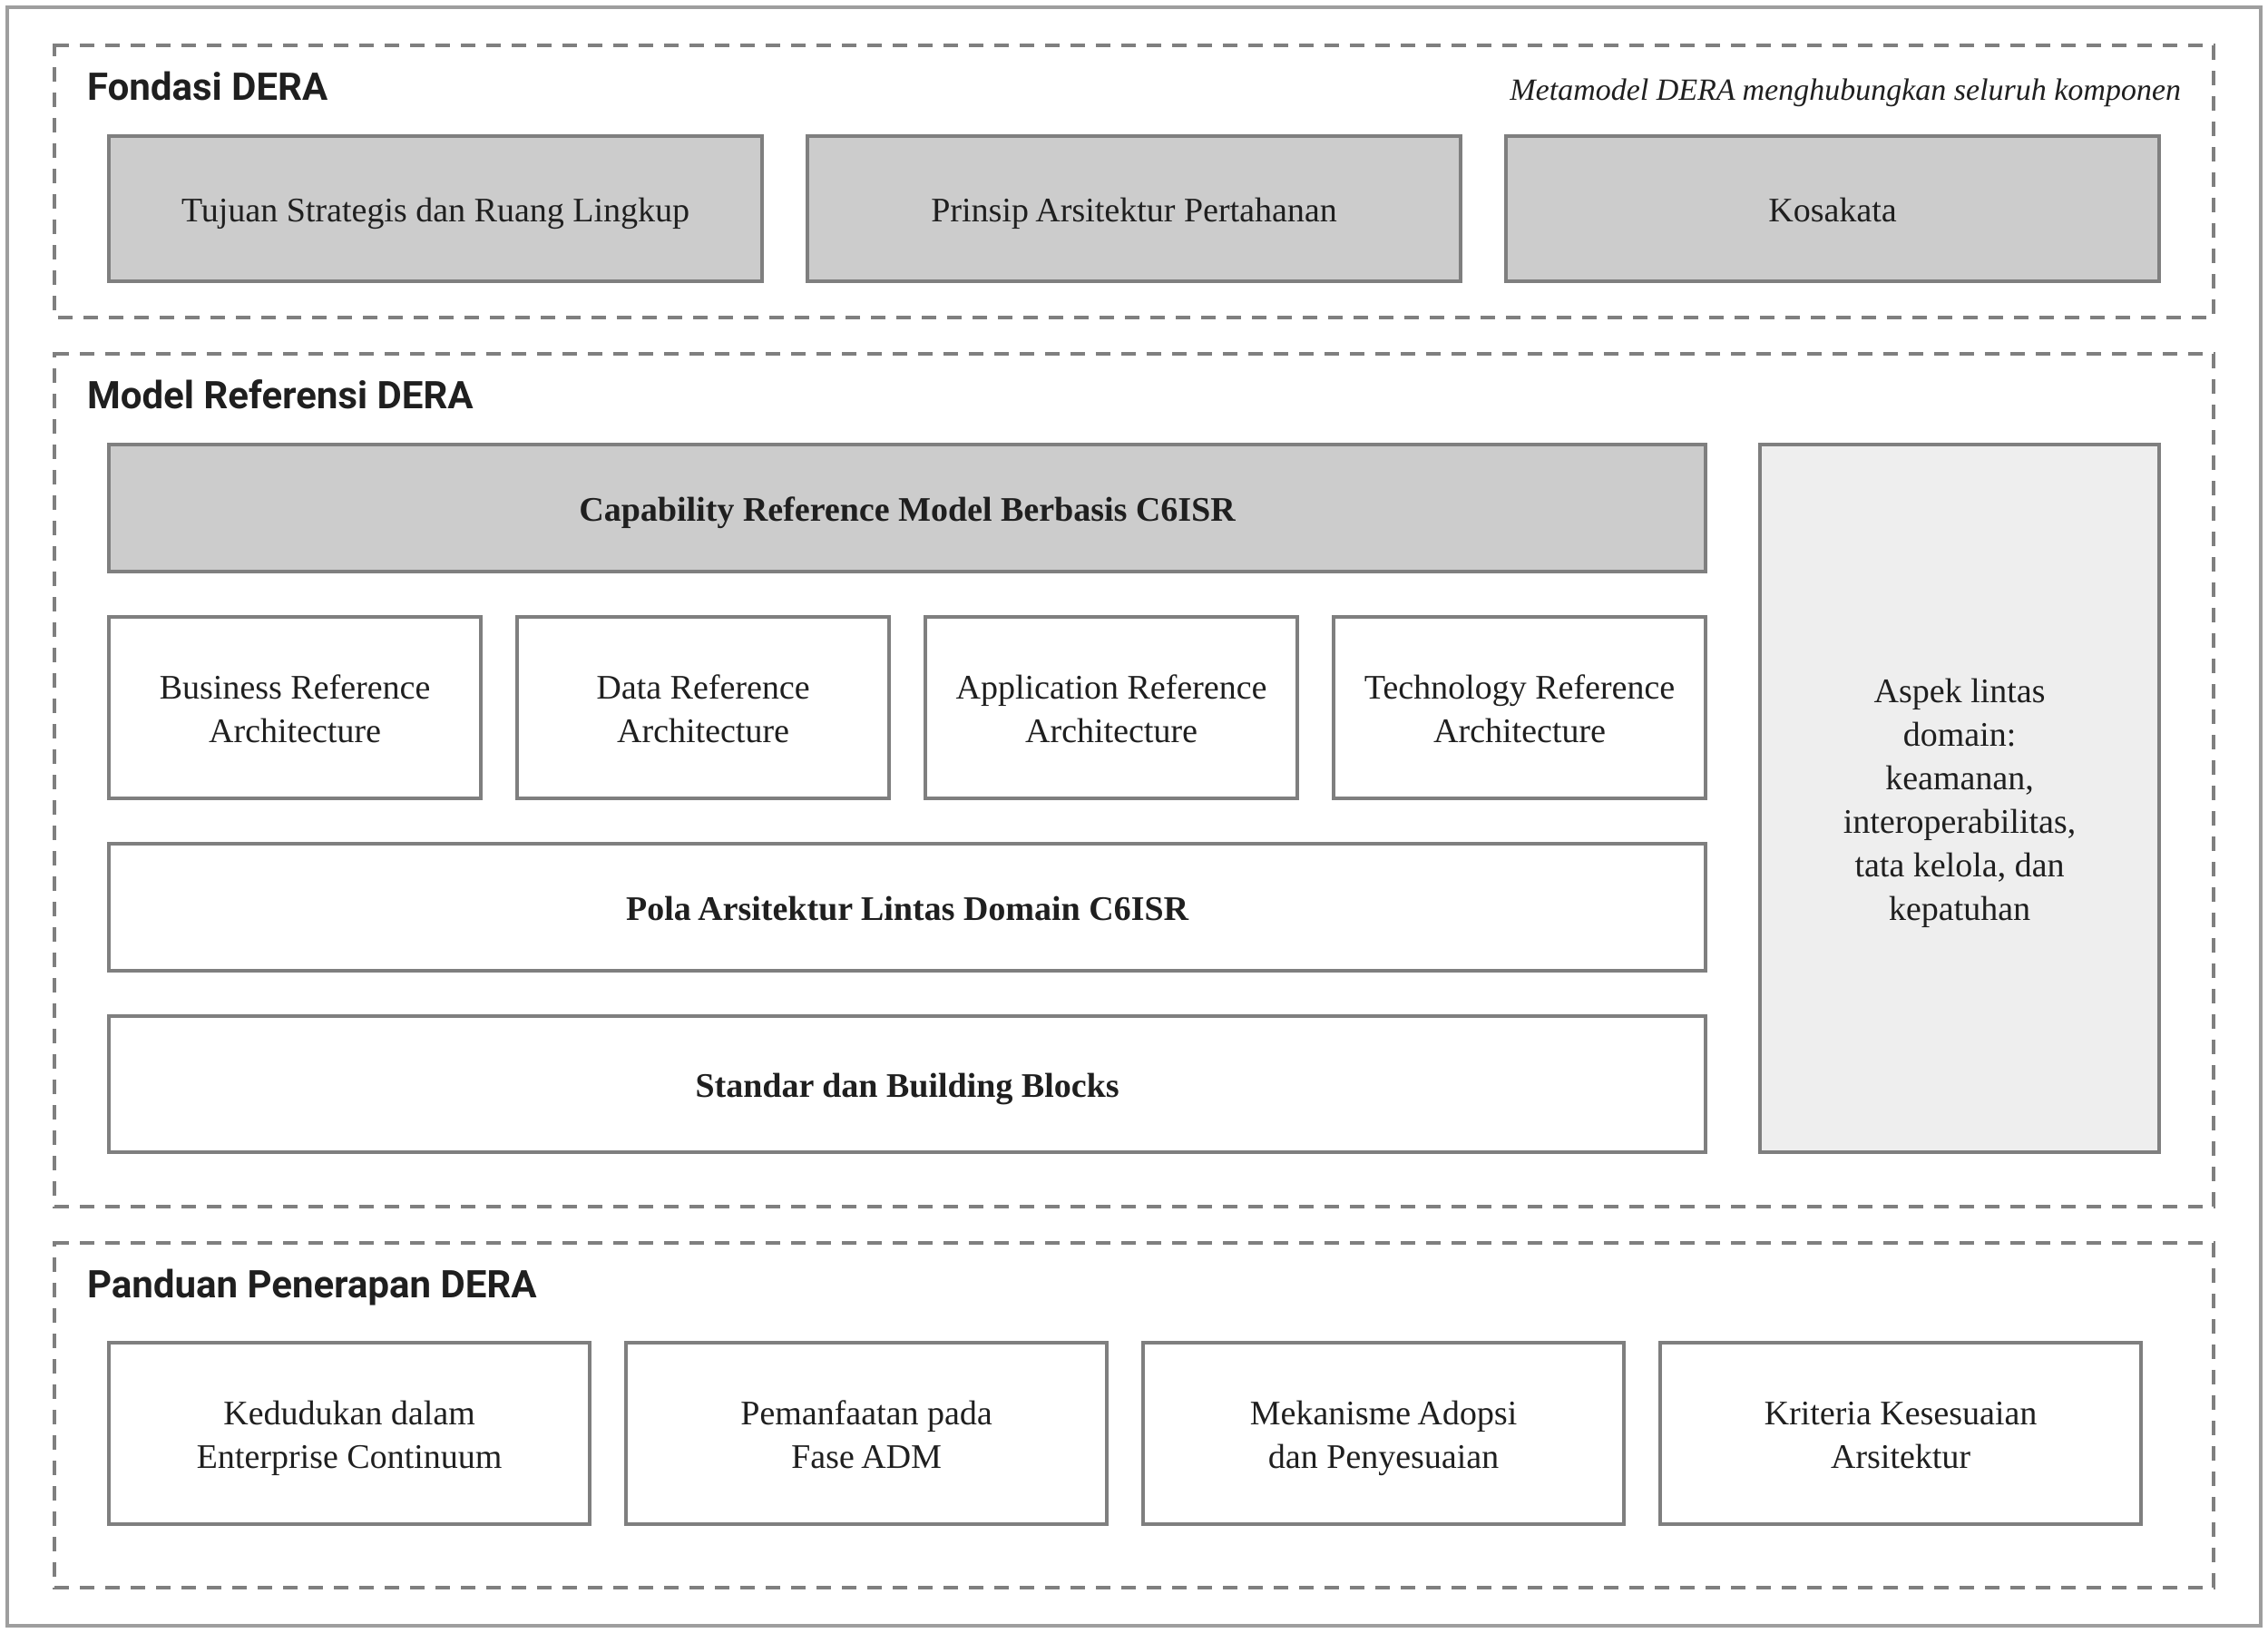
\includegraphics[width=1.00\linewidth,height=0.8\textheight,keepaspectratio]{images/Struktur DERA.png}
\caption{Struktur DERA}
\label{fig:III.2}
\end{figure}

Gambar~\ref{fig:III.2} menunjukkan bahwa lapisan fondasi memuat tujuan strategis dan ruang lingkup, prinsip arsitektur pertahanan, serta kosakata. Lapisan model referensi memuat \textit{Capability Reference Model} berbasis C6ISR, arsitektur referensi empat domain, pola lintas domain C6ISR, serta standar dan \textit{building blocks}, dengan aspek keamanan, interoperabilitas, tata kelola, dan kepatuhan sebagai aspek lintas domain. Lapisan panduan penerapan memuat kedudukan DERA dalam \textit{Enterprise Continuum}, pemanfaatannya pada fase ADM, mekanisme adopsi dan penyesuaian, serta kriteria kesesuaian arsitektur. Dengan struktur tersebut, kelima komponen arsitektur referensi terpenuhi, yaitu tujuan strategis, prinsip, dan kosakata pada lapis fondasi, serta posisi teknis dan pola pada lapis model referensi \cite{DoDCIO2010RA}.

Komponen DERA dihubungkan oleh metamodel DERA, yaitu model yang mendefinisikan jenis entitas dan hubungan antarentitas, sebagaimana dianjurkan TOGAF melalui \textit{enterprise metamodel} \cite{TOGAF2022}. Entitas dan hubungan utama metamodel DERA disajikan pada Tabel~\ref{tab:III.8}.

\begingroup\small\setstretch{1.0}
\begin{longtable}{@{}>{\raggedright\arraybackslash\hspace{0pt}}p{0.313\linewidth}>{\raggedright\arraybackslash\hspace{0pt}}p{0.284\linewidth}>{\raggedright\arraybackslash\hspace{0pt}}p{0.341\linewidth}@{}}
\caption{Entitas dan Hubungan Utama Metamodel DERA}\label{tab:III.8}\\
\toprule
\textbf{Entitas Asal} & \textbf{Hubungan} & \textbf{Entitas Tujuan}\\
\midrule
\endfirsthead
\multicolumn{3}{@{}l}{\small\itshape \tablename\ \thetable{} (lanjutan)}\\
\toprule
\textbf{Entitas Asal} & \textbf{Hubungan} & \textbf{Entitas Tujuan}\\
\midrule
\endhead
\bottomrule
\endlastfoot
Unsur C6ISR & diwujudkan oleh & Kapabilitas\\*
Kapabilitas & direalisasikan oleh & Proses dan layanan bisnis\\
Proses bisnis & dijalankan oleh & Peran dan unit organisasi\\
Proses bisnis & menggunakan dan menghasilkan & Entitas data\\
Proses dan layanan bisnis & didukung oleh & Layanan aplikasi\\
Komponen aplikasi & mengelola & Entitas data\\
Komponen aplikasi & berjalan pada & Layanan teknologi\\
Prinsip & mengarahkan & Seluruh komponen DERA\\
Standar (posisi teknis) & membatasi & \textit{Building block}\\
Pola & memadukan & Elemen lintas domain\\
Kebutuhan arsitektur referensi & dipenuhi oleh & Komponen DERA\\
Aliran nilai & didukung oleh & Kapabilitas\\
Area subjek data & mengelompokkan & Entitas data\\*
Layanan teknologi & mewujudkan & Unsur C6ISR (\textit{communications}, \textit{computers}, \textit{cyber-defense})\\
\end{longtable}
\endgroup

Tabel~\ref{tab:III.8} menunjukkan bahwa metamodel DERA menghubungkan unsur C6ISR hingga layanan teknologi dalam satu rantai, serta menautkan setiap komponen dengan kebutuhan arsitektur referensi. Metamodel tersebut menjadi dasar aturan konsistensi dan matriks keterlacakan pada evaluasi Bab V.

\section{Fondasi DERA}
\label{sec:III.3}

Fondasi DERA memuat tiga komponen arsitektur referensi yang mengarahkan seluruh komponen lainnya, yaitu tujuan strategis dan ruang lingkup, prinsip arsitektur, serta kosakata.

\subsection{Tujuan Strategis dan Ruang Lingkup}
\label{sec:III.3.1}

Tujuan strategis DERA adalah menjadi acuan bersama dalam pengembangan EA di lingkungan pertahanan Indonesia, dengan sasaran sebagai berikut.

\begin{enumerate}[label=\arabic*.]
\item Menyatukan arah pengembangan EA lintas organisasi pertahanan agar \textit{silo} tidak berpindah ke tingkat arsitektur.
\item Menjamin interoperabilitas dan keamanan sejak tahap perancangan.
\item Menautkan investasi digital dengan kapabilitas C6ISR serta doktrin dan strategi pertahanan.
\item Menyelaraskan arsitektur pertahanan dengan Arsitektur SPBE dan regulasi nasional.
\end{enumerate}

Ruang lingkup DERA ditetapkan sebagai berikut. Dari sisi pengguna, Kemhan RI berperan sebagai penetap dan pemelihara DERA, Mabes TNI dan ketiga matra sebagai pengguna, serta industri pertahanan sebagai mitra yang menyesuaikan antarmukanya. Dari sisi cakupan, DERA mencakup domain bisnis, data, aplikasi, dan teknologi pada tingkat EA, kebijakan, dan standar. DERA tidak mencakup desain teknis sistem senjata, prosedur operasi, maupun informasi rahasia militer.

\subsection{Prinsip Arsitektur Pertahanan}
\label{sec:III.3.2}

Prinsip arsitektur mengarahkan keputusan perancangan pada seluruh arsitektur turunan agar konsisten. Prinsip dikembangkan dari sembilan prinsip pertahanan dan dilengkapi rasional, implikasi, serta keterlacakan terhadap kebutuhan arsitektur referensi, sebagaimana disajikan pada Tabel~\ref{tab:III.9}.

\begingroup\small\setstretch{1.0}
\begin{longtable}{@{}>{\raggedright\arraybackslash\hspace{0pt}}p{0.182\linewidth}>{\raggedright\arraybackslash\hspace{0pt}}p{0.204\linewidth}>{\raggedright\arraybackslash\hspace{0pt}}p{0.188\linewidth}>{\raggedright\arraybackslash\hspace{0pt}}p{0.208\linewidth}>{\raggedright\arraybackslash\hspace{0pt}}p{0.094\linewidth}@{}}
\caption{Prinsip Arsitektur Pertahanan}\label{tab:III.9}\\
\toprule
\textbf{Prinsip} & \textbf{Pernyataan} & \textbf{Rasional} & \textbf{Implikasi} & \textbf{KR}\\
\midrule
\endfirsthead
\multicolumn{5}{@{}l}{\small\itshape \tablename\ \thetable{} (lanjutan)}\\
\toprule
\textbf{Prinsip} & \textbf{Pernyataan} & \textbf{Rasional} & \textbf{Implikasi} & \textbf{KR}\\
\midrule
\endhead
\bottomrule
\endlastfoot
1. \textit{Interoperability} & Sistem organisasi pertahanan dapat bertukar data dan layanan melalui standar bersama. & Perencanaan dan operasi pertahanan melibatkan banyak entitas. & Pengembangan sistem wajib mengikuti standar antarmuka dan pertukaran data DERA. & KR-04\\*
2. \textit{Security by Design} & Keamanan siber dan klasifikasi informasi ditetapkan sejak perancangan. & Data dan sistem pertahanan menjadi sasaran ancaman siber. & Setiap komponen memiliki klasifikasi dan kendali keamanan sejak tahap desain. & KR-03\\
3. \textit{Data as Strategic Asset} & Data pertahanan dikelola sebagai aset strategis. & Keunggulan informasi menentukan keunggulan operasi. & Setiap entitas data memiliki pemilik, kamus data, metadata, dan klasifikasi. & KR-02, KR-06\\
4. \textit{Integrated Command \& Control} & Arsitektur mendukung komando dan kendali yang terpadu lintas tingkat dan lintas matra. & Efektivitas operasi bergantung pada keterpaduan siklus C6ISR. & Kapabilitas dan aplikasi komando-kendali berbagi gambaran situasi yang sama. & KR-01\\
5. \textit{Availability \& Reliability} & Layanan pertahanan kritis tetap tersedia ketika terjadi gangguan. & Operasi tidak boleh bergantung pada satu titik kegagalan. & Diperlukan redundansi pusat data, jalur komunikasi berlapis, dan kemampuan beroperasi terputus. & KR-01, KR-03\\
6. \textit{Scalability \& Flexibility} & Arsitektur dapat berkembang mengikuti perubahan ancaman, teknologi, dan organisasi. & Lingkungan strategis dan teknologi berubah cepat. & Komponen dirancang modular dengan titik variasi yang jelas. & KR-09\\
7. \textit{Governance \& Compliance} & Arsitektur tunduk pada tata kelola arsitektur dan regulasi nasional. & Organisasi pertahanan wajib memenuhi SPBE, Satu Data, dan ketentuan keamanan siber. & Arsitektur turunan diperiksa kesesuaiannya terhadap DERA dan regulasi. & KR-06, KR-10\\
8. \textit{Smart Defence Oriented} & Transformasi digital diarahkan untuk mendukung doktrin, strategi, dan pertahanan cerdas. & Investasi digital harus mendukung tujuan pertahanan, bukan kebutuhan unit semata. & Setiap inisiatif ditelusuri ke sasaran strategis pertahanan. & KR-05\\*
9. \textit{User-Centric Service} & Layanan digital dirancang berdasarkan kebutuhan pengguna. & Efektivitas personel menentukan keberhasilan transformasi. & Layanan bersama dan akses tunggal diutamakan dibandingkan aplikasi per unit. & KR-02\\
\end{longtable}
\endgroup

Tabel~\ref{tab:III.9} menunjukkan bahwa setiap prinsip dapat ditelusuri ke kebutuhan arsitektur referensi, dan setiap kebutuhan muatan pertahanan, yaitu KR-01, KR-03, KR-04, dan KR-05, memiliki prinsip yang mengikat.

\subsection{Kosakata}
\label{sec:III.3.3}

Kosakata DERA menyamakan pemahaman istilah antara penyusun dan pengguna arsitektur turunan. Istilah utama DERA disajikan pada Tabel~\ref{tab:III.10}.

\begingroup\small\setstretch{1.0}
\begin{longtable}{@{}>{\raggedright\arraybackslash\hspace{0pt}}p{0.281\linewidth}>{\raggedright\arraybackslash\hspace{0pt}}p{0.688\linewidth}@{}}
\caption{Kosakata Utama DERA}\label{tab:III.10}\\
\toprule
\textbf{Istilah} & \textbf{Definisi}\\
\midrule
\endfirsthead
\multicolumn{2}{@{}l}{\small\itshape \tablename\ \thetable{} (lanjutan)}\\
\toprule
\textbf{Istilah} & \textbf{Definisi}\\
\midrule
\endhead
\bottomrule
\endlastfoot
Arsitektur referensi & Arsitektur generik yang mengarahkan dan membatasi arsitektur organisasi dalam satu kelas organisasi.\\*
Arsitektur turunan & Arsitektur organisasi pertahanan yang disusun dengan mengacu pada DERA.\\
Kapabilitas & Kemampuan organisasi untuk mencapai hasil tertentu, terlepas dari unit atau sistem yang melaksanakannya.\\
Unsur C6ISR & Salah satu dari sembilan unsur dalam definisi operasional C6ISR.\\
Siklus C6ISR & Rangkaian pengindraan, pemahaman situasi, keputusan, penindakan, dan penilaian.\\
Gambaran situasi bersama & Tampilan situasi operasional yang sama bagi seluruh tingkat komando sesuai hak aksesnya.\\
Pola lintas domain & Solusi generik yang memadukan elemen bisnis, data, aplikasi, dan teknologi untuk satu fungsi C6ISR.\\
Posisi teknis & Standar atau ketentuan teknis yang wajib diikuti arsitektur turunan.\\
\textit{Building block} & Komponen arsitektur yang dapat digunakan ulang dan memiliki antarmuka yang jelas.\\
Titik variasi & Bagian DERA yang dapat disesuaikan oleh arsitektur turunan.\\
Domain klasifikasi & Lingkungan jaringan dan sistem yang memproses informasi dengan tingkat klasifikasi yang sama.\\
Proses dan layanan bisnis & Aktivitas dan layanan organisasi yang merealisasikan kapabilitas.\\
Peran dan unit organisasi & Pihak yang menjalankan proses bisnis.\\
Entitas data & Objek data yang digunakan dan dihasilkan proses bisnis serta dikelola komponen aplikasi.\\
Layanan aplikasi & Fungsi aplikasi yang mendukung proses dan layanan bisnis.\\
Komponen aplikasi & Satuan perangkat lunak yang menyediakan layanan aplikasi dan mengelola entitas data.\\
Layanan teknologi & Layanan infrastruktur tempat komponen aplikasi berjalan.\\
Prinsip arsitektur & Ketentuan umum yang mengarahkan keputusan perancangan arsitektur.\\
Kebutuhan arsitektur referensi (KR) & Kebutuhan yang harus dipenuhi DERA sebagai arsitektur referensi pertahanan.\\
Aliran nilai & Rangkaian tahapan yang menghasilkan nilai bagi pemangku kepentingan.\\
Area subjek data & Kelompok entitas data dengan pokok bahasan yang sama.\\*
Gerbang lintas domain & Komponen yang mengendalikan pertukaran data antardomain klasifikasi.\\
\end{longtable}
\endgroup

\section{Model Referensi DERA}
\label{sec:III.4}

Model referensi DERA menerjemahkan fondasi DERA ke dalam kapabilitas, empat domain arsitektur, pola lintas domain, aspek lintas domain, serta standar dan \textit{building blocks}.

\subsection{Capability Reference Model Berbasis C6ISR}
\label{sec:III.4.1}

\textit{Capability Reference Model} (CRM\label{sk:CRM}) memetakan kapabilitas yang dibutuhkan organisasi pertahanan, tanpa bergantung pada unit atau sistem yang melaksanakannya. CRM menggabungkan kapabilitas operasional C6ISR dengan kapabilitas strategis dan pengelolaan sumber daya, karena kementerian pertahanan menjalankan fungsi kebijakan, pengadaan, dan pengelolaan sumber daya nasional \cite{UU3Tahun2002}. Struktur CRM ditunjukkan pada Gambar~\ref{fig:III.3}.

\begin{figure}[htbp]
\centering
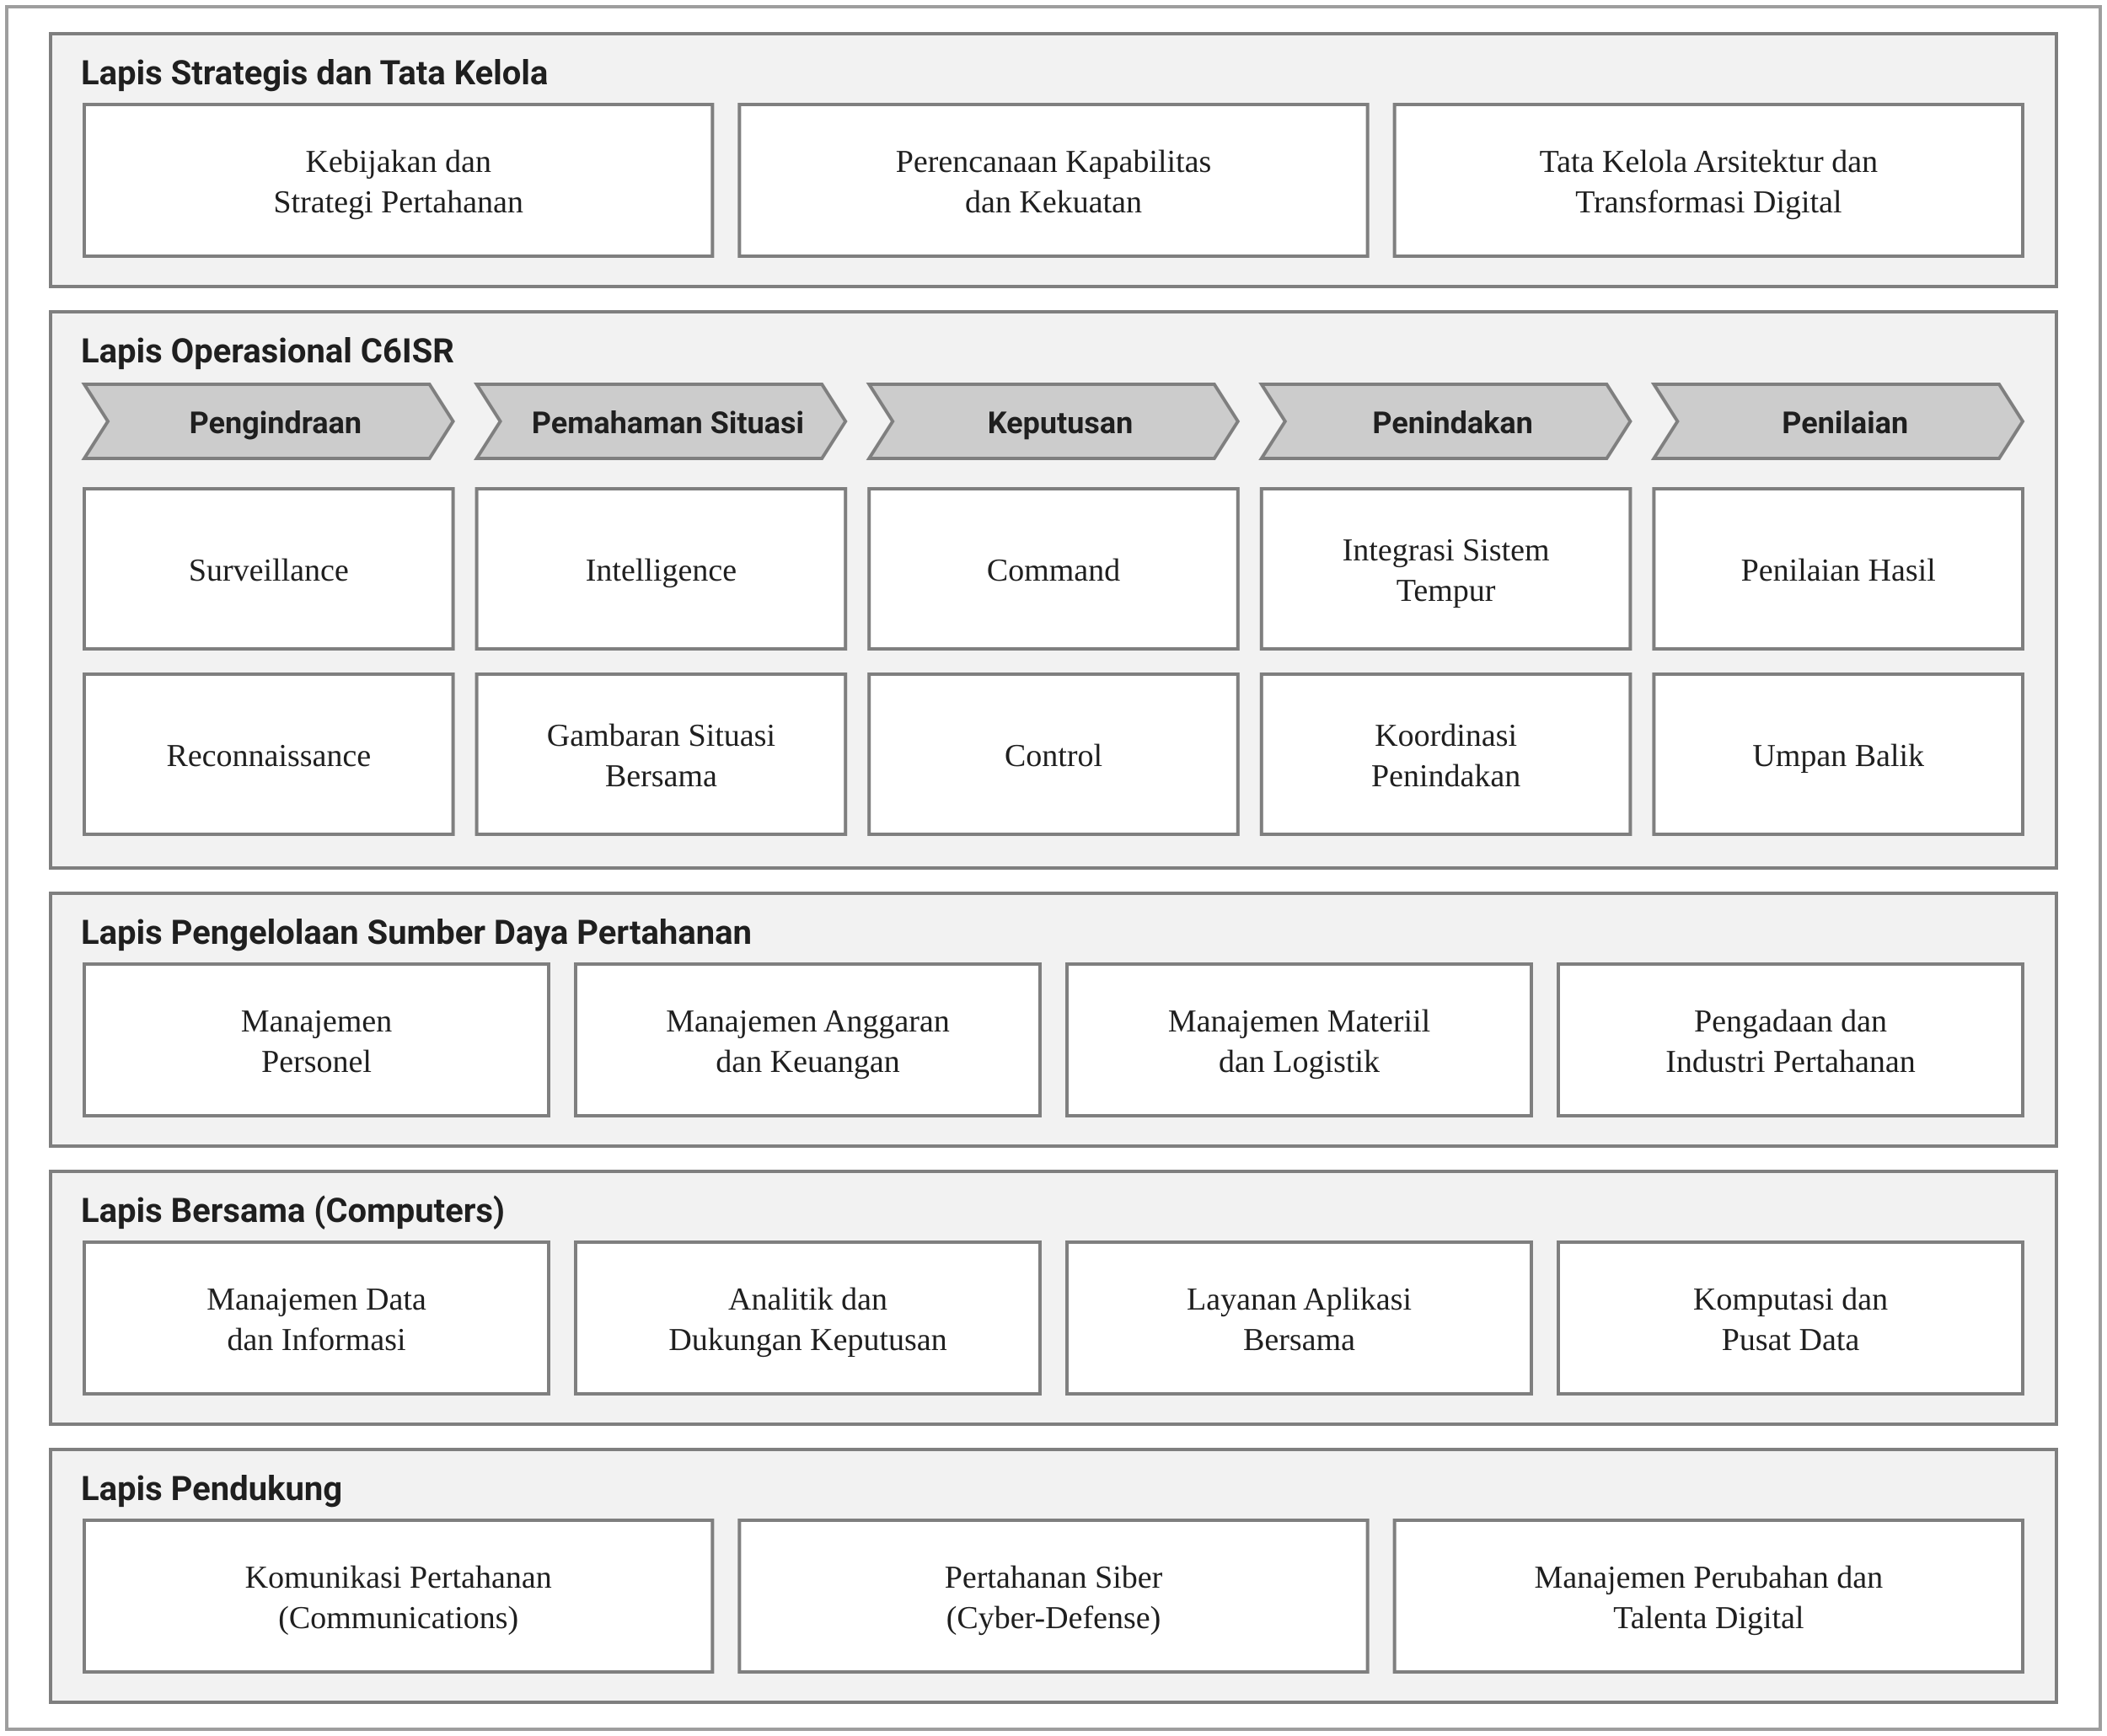
\includegraphics[width=1.00\linewidth,height=0.8\textheight,keepaspectratio]{images/Capability Reference Model DERA.png}
\caption{\textit{Capability Reference Model} DERA}
\label{fig:III.3}
\end{figure}

Gambar~\ref{fig:III.3} menunjukkan bahwa CRM terdiri atas lima lapis. Lapis operasional C6ISR disusun mengikuti siklus pengindraan, pemahaman situasi, keputusan, penindakan, dan penilaian, sehingga keterpaduan siklus C6ISR terjaga sebagai rantai kapabilitas. Peran setiap lapis dan unsur C6ISR terkait disajikan pada Tabel~\ref{tab:III.11}.

\begingroup\small\setstretch{1.0}
\begin{longtable}{@{}>{\raggedright\arraybackslash\hspace{0pt}}p{0.272\linewidth}>{\raggedright\arraybackslash\hspace{0pt}}p{0.406\linewidth}>{\raggedright\arraybackslash\hspace{0pt}}p{0.260\linewidth}@{}}
\caption{Lapis \textit{Capability Reference Model} dan Unsur C6ISR}\label{tab:III.11}\\
\toprule
\textbf{Lapis} & \textbf{Peran} & \textbf{Unsur C6ISR Terkait}\\
\midrule
\endfirsthead
\multicolumn{3}{@{}l}{\small\itshape \tablename\ \thetable{} (lanjutan)}\\
\toprule
\textbf{Lapis} & \textbf{Peran} & \textbf{Unsur C6ISR Terkait}\\
\midrule
\endhead
\bottomrule
\endlastfoot
Strategis dan tata kelola & Menetapkan arah, perencanaan kapabilitas, dan tata kelola arsitektur. & \textit{Command} (tingkat strategis)\\*
Operasional C6ISR & Menjalankan siklus operasi dari pengindraan hingga penilaian. & \textit{Intelligence}, \textit{Surveillance}, \textit{Reconnaissance}, \textit{Command}, \textit{Control}, \textit{Combat Systems}\\
Pengelolaan sumber daya pertahanan & Mengelola personel, anggaran, materiil, dan pengadaan. & \textit{Combat Systems} (pengadaan alutsista)\\
Bersama & Menyediakan data, analitik, aplikasi, dan komputasi bagi seluruh lapis. & \textit{Computers}\\*
Pendukung & Menyediakan komunikasi, pertahanan siber, dan kesiapan perubahan. & \textit{Communications}, \textit{Cyber-Defense}\\
\end{longtable}
\endgroup

Tabel~\ref{tab:III.11} menunjukkan bahwa kesembilan unsur C6ISR terwakili dalam CRM. Kapabilitas Tata Kelola Arsitektur dan Transformasi Digital serta Manajemen Perubahan dan Talenta Digital ditambahkan karena tantangan tata kelola dan SDM pada Tabel~\ref{tab:II.1} menyebabkan pengembangan sistem berjalan sendiri-sendiri.

\subsection{Business Reference Architecture}
\label{sec:III.4.2}

\textit{Business Reference Architecture} (BRA\label{sk:BRA}) menyediakan acuan entitas, aliran nilai, layanan bisnis, dan tata kelola yang digunakan arsitektur turunan untuk menyusun arsitektur bisnis. Elemen BRA disajikan pada Tabel~\ref{tab:III.12}.

\begingroup\small\setstretch{1.0}
\begin{longtable}{@{}>{\raggedright\arraybackslash\hspace{0pt}}p{0.257\linewidth}>{\raggedright\arraybackslash\hspace{0pt}}p{0.712\linewidth}@{}}
\caption{Elemen \textit{Business Reference Architecture}}\label{tab:III.12}\\
\toprule
\textbf{Elemen} & \textbf{Isi Acuan}\\
\midrule
\endfirsthead
\multicolumn{2}{@{}l}{\small\itshape \tablename\ \thetable{} (lanjutan)}\\
\toprule
\textbf{Elemen} & \textbf{Isi Acuan}\\
\midrule
\endhead
\bottomrule
\endlastfoot
Entitas dan peran & Kementerian pertahanan sebagai penetap kebijakan dan standar; markas besar angkatan bersenjata sebagai pengendali operasi; matra sebagai pelaksana; industri pertahanan sebagai mitra penyedia alutsista.\\*
Aliran nilai & Perumusan kebijakan dan strategi; pengembangan kekuatan dan kapabilitas; pelaksanaan operasional dan dukungan; tata kelola, pengawasan, dan kepatuhan; serta pengelolaan sumber daya dan aset pertahanan.\\
Layanan bisnis & Layanan kebijakan dan perencanaan, layanan pengelolaan sumber daya, layanan dukungan operasi, layanan informasi pertahanan, serta layanan pengembangan organisasi dan talenta digital.\\
Tata kelola komando & Komando dan kendali berjenjang pada tingkat strategis, operasional, dan pelaksana (pola P2).\\*
Tata kelola arsitektur & Fungsi pemilik arsitektur di tingkat kementerian, dewan arsitektur, dan tinjauan kesesuaian arsitektur turunan.\\
\end{longtable}
\endgroup

Tabel~\ref{tab:III.12} menunjukkan bahwa BRA memisahkan peran penetap kebijakan dan pengendali operasi. Pemisahan tersebut menjaga agar arsitektur turunan tidak memodelkan prosedur operasi, tetapi menyediakan kebijakan, standar, dan layanan yang memungkinkan operasi terpadu.

\subsection{Data Reference Architecture}
\label{sec:III.4.3}

\textit{Data Reference Architecture} (DRA\label{sk:DRA}) menyediakan acuan area subjek data, klasifikasi, dan tata kelola data. Area subjek data pertahanan disajikan pada Tabel~\ref{tab:III.13}.

\begingroup\small\setstretch{1.0}
\begin{longtable}{@{}>{\raggedright\arraybackslash\hspace{0pt}}p{0.248\linewidth}>{\raggedright\arraybackslash\hspace{0pt}}p{0.418\linewidth}>{\raggedright\arraybackslash\hspace{0pt}}p{0.272\linewidth}@{}}
\caption{Area Subjek Data Pertahanan}\label{tab:III.13}\\
\toprule
\textbf{Area Subjek} & \textbf{Contoh Entitas Data} & \textbf{Klasifikasi Acuan}\\
\midrule
\endfirsthead
\multicolumn{3}{@{}l}{\small\itshape \tablename\ \thetable{} (lanjutan)}\\
\toprule
\textbf{Area Subjek} & \textbf{Contoh Entitas Data} & \textbf{Klasifikasi Acuan}\\
\midrule
\endhead
\bottomrule
\endlastfoot
Kebijakan dan strategi & Kebijakan, rencana strategis, sasaran kapabilitas & Terbatas–Rahasia\\*
Personel & Data personel, kompetensi, penugasan & Terbatas\\
Anggaran dan keuangan & Pagu, realisasi, aset keuangan & Terbuka–Terbatas\\
Materiil dan alutsista & Inventaris, status kesiapan, pemeliharaan & Terbatas–Rahasia\\
Operasi dan situasi & Rencana operasi, laporan situasi, status kekuatan & Rahasia\\
Intelijen dan ISR & Data sensor, produk intelijen, penilaian ancaman & Rahasia\\
Geospasial & Peta dasar, wilayah pertahanan, titik pantau & Terbuka–Rahasia\\
Infrastruktur dan TIK & Aset TIK, konfigurasi, log keamanan & Terbatas\\
Industri pertahanan & Penyedia, kontrak, kemampuan produksi & Terbuka–Terbatas\\*
Informasi publik & Informasi dan layanan publik pertahanan & Terbuka\\
\end{longtable}
\endgroup

Tabel~\ref{tab:III.13} menunjukkan klasifikasi acuan setiap area subjek berdasarkan tiga tingkat klasifikasi, yaitu Terbuka, Terbatas, dan Rahasia. Klasifikasi akhir setiap entitas ditetapkan oleh pemilik data pada arsitektur turunan. Tata kelola data mengikuti peran penyelenggara Satu Data Pertahanan, yaitu pengarah, walidata, produsen data, pengolah data, dan pengaman sistem data. Setiap area subjek dilengkapi kamus data yang mendefinisikan entitas dan atributnya, sedangkan metadata melekat pada setiap \textit{dataset}.

\subsection{Application Reference Architecture}
\label{sec:III.4.4}

\textit{Application Reference Architecture} (ARA\label{sk:ARA}) mengelompokkan aplikasi berdasarkan fungsi dan domain klasifikasinya, sebagaimana disajikan pada Tabel~\ref{tab:III.14}.

\begingroup\small\setstretch{1.0}
\begin{longtable}{@{}>{\raggedright\arraybackslash\hspace{0pt}}p{0.260\linewidth}>{\raggedright\arraybackslash\hspace{0pt}}p{0.453\linewidth}>{\raggedright\arraybackslash\hspace{0pt}}p{0.225\linewidth}@{}}
\caption{Kategori \textit{Application Reference Architecture}}\label{tab:III.14}\\
\toprule
\textbf{Kategori} & \textbf{Layanan Aplikasi Acuan} & \textbf{Domain Klasifikasi}\\
\midrule
\endfirsthead
\multicolumn{3}{@{}l}{\small\itshape \tablename\ \thetable{} (lanjutan)}\\
\toprule
\textbf{Kategori} & \textbf{Layanan Aplikasi Acuan} & \textbf{Domain Klasifikasi}\\
\midrule
\endhead
\bottomrule
\endlastfoot
Aplikasi umum SPBE & Aplikasi nasional yang digunakan bersama instansi pemerintah & Administrasi\\*
Aplikasi administrasi pertahanan & Personel, keuangan, materiil dan logistik, serta pengadaan & Administrasi\\
Aplikasi operasional C6ISR & Komando-kendali, gambaran situasi bersama, fusi data, perencanaan operasi, dan pengelolaan sensor & Operasional\\
Aplikasi bersama pertahanan & Identitas tunggal, kolaborasi, portal dan katalog data, serta analitik dan dasbor & Administrasi\\*
Layanan integrasi & Pertukaran data, antarmuka pemrograman aplikasi, dan gerbang lintas domain & Administrasi dan operasional\\
\end{longtable}
\endgroup

Tabel~\ref{tab:III.14} menunjukkan bahwa aplikasi umum SPBE digunakan sesuai ketentuan pemiliknya dan tidak dikembangkan ulang, sedangkan aplikasi khusus pertahanan dikelompokkan berdasarkan fungsi. Aplikasi dengan fungsi serupa diarahkan menjadi aplikasi bersama, dan seluruh pertukaran data dilakukan melalui layanan integrasi.

\subsection{Technology Reference Architecture}
\label{sec:III.4.5}

\textit{Technology Reference Architecture} (TRA\label{sk:TRA}) menyediakan acuan kategori layanan teknologi yang menopang aplikasi dan data, sebagaimana disajikan pada Tabel~\ref{tab:III.15}.

\begingroup\small\setstretch{1.0}
\begin{longtable}{@{}>{\raggedright\arraybackslash\hspace{0pt}}p{0.272\linewidth}>{\raggedright\arraybackslash\hspace{0pt}}p{0.441\linewidth}>{\raggedright\arraybackslash\hspace{0pt}}p{0.225\linewidth}@{}}
\caption{Kategori \textit{Technology Reference Architecture}}\label{tab:III.15}\\
\toprule
\textbf{Kategori} & \textbf{Layanan Teknologi Acuan} & \textbf{Unsur C6ISR}\\
\midrule
\endfirsthead
\multicolumn{3}{@{}l}{\small\itshape \tablename\ \thetable{} (lanjutan)}\\
\toprule
\textbf{Kategori} & \textbf{Layanan Teknologi Acuan} & \textbf{Unsur C6ISR}\\
\midrule
\endhead
\bottomrule
\endlastfoot
Pusat data dan pemulihan bencana & Pusat data utama dan pusat pemulihan bencana dengan mode aktif-aktif & \textit{Computers}\\*
Komputasi \textit{edge} dan platform & Komputasi di pangkalan, pusat komando wilayah, dan platform & \textit{Computers}\\
Jaringan administrasi & Jaringan untuk informasi Terbuka dan Terbatas & \textit{Communications}\\
Jaringan operasional terklasifikasi & Jaringan terpisah untuk informasi Rahasia & \textit{Communications}, \textit{Cyber-Defense}\\
Komunikasi strategis dan taktis & Serat optik, satelit, radio, dan jalur cadangan & \textit{Communications}\\
Layanan platform bersama & Identitas, integrasi, dan platform data & \textit{Computers}\\
Keamanan teknologi & Pusat operasi keamanan, persandian, dan gerbang lintas domain & \textit{Cyber-Defense}\\*
Manajemen layanan TI & Pemantauan, manajemen insiden, dan manajemen konfigurasi & \textit{Computers}\\
\end{longtable}
\endgroup

Tabel~\ref{tab:III.15} menunjukkan bahwa TRA memisahkan jaringan administrasi dan jaringan operasional terklasifikasi. Pemisahan tersebut merupakan dasar pola pemisahan domain klasifikasi pada III.4.6.

\subsection{Pola Arsitektur Lintas Domain C6ISR}
\label{sec:III.4.6}

Pola lintas domain memadukan elemen keempat domain untuk setiap fungsi C6ISR, sehingga keterpaduan siklus C6ISR tetap terjaga. Keenam pola DERA ditunjukkan pada Gambar~\ref{fig:III.4}.

\begin{figure}[htbp]
\centering
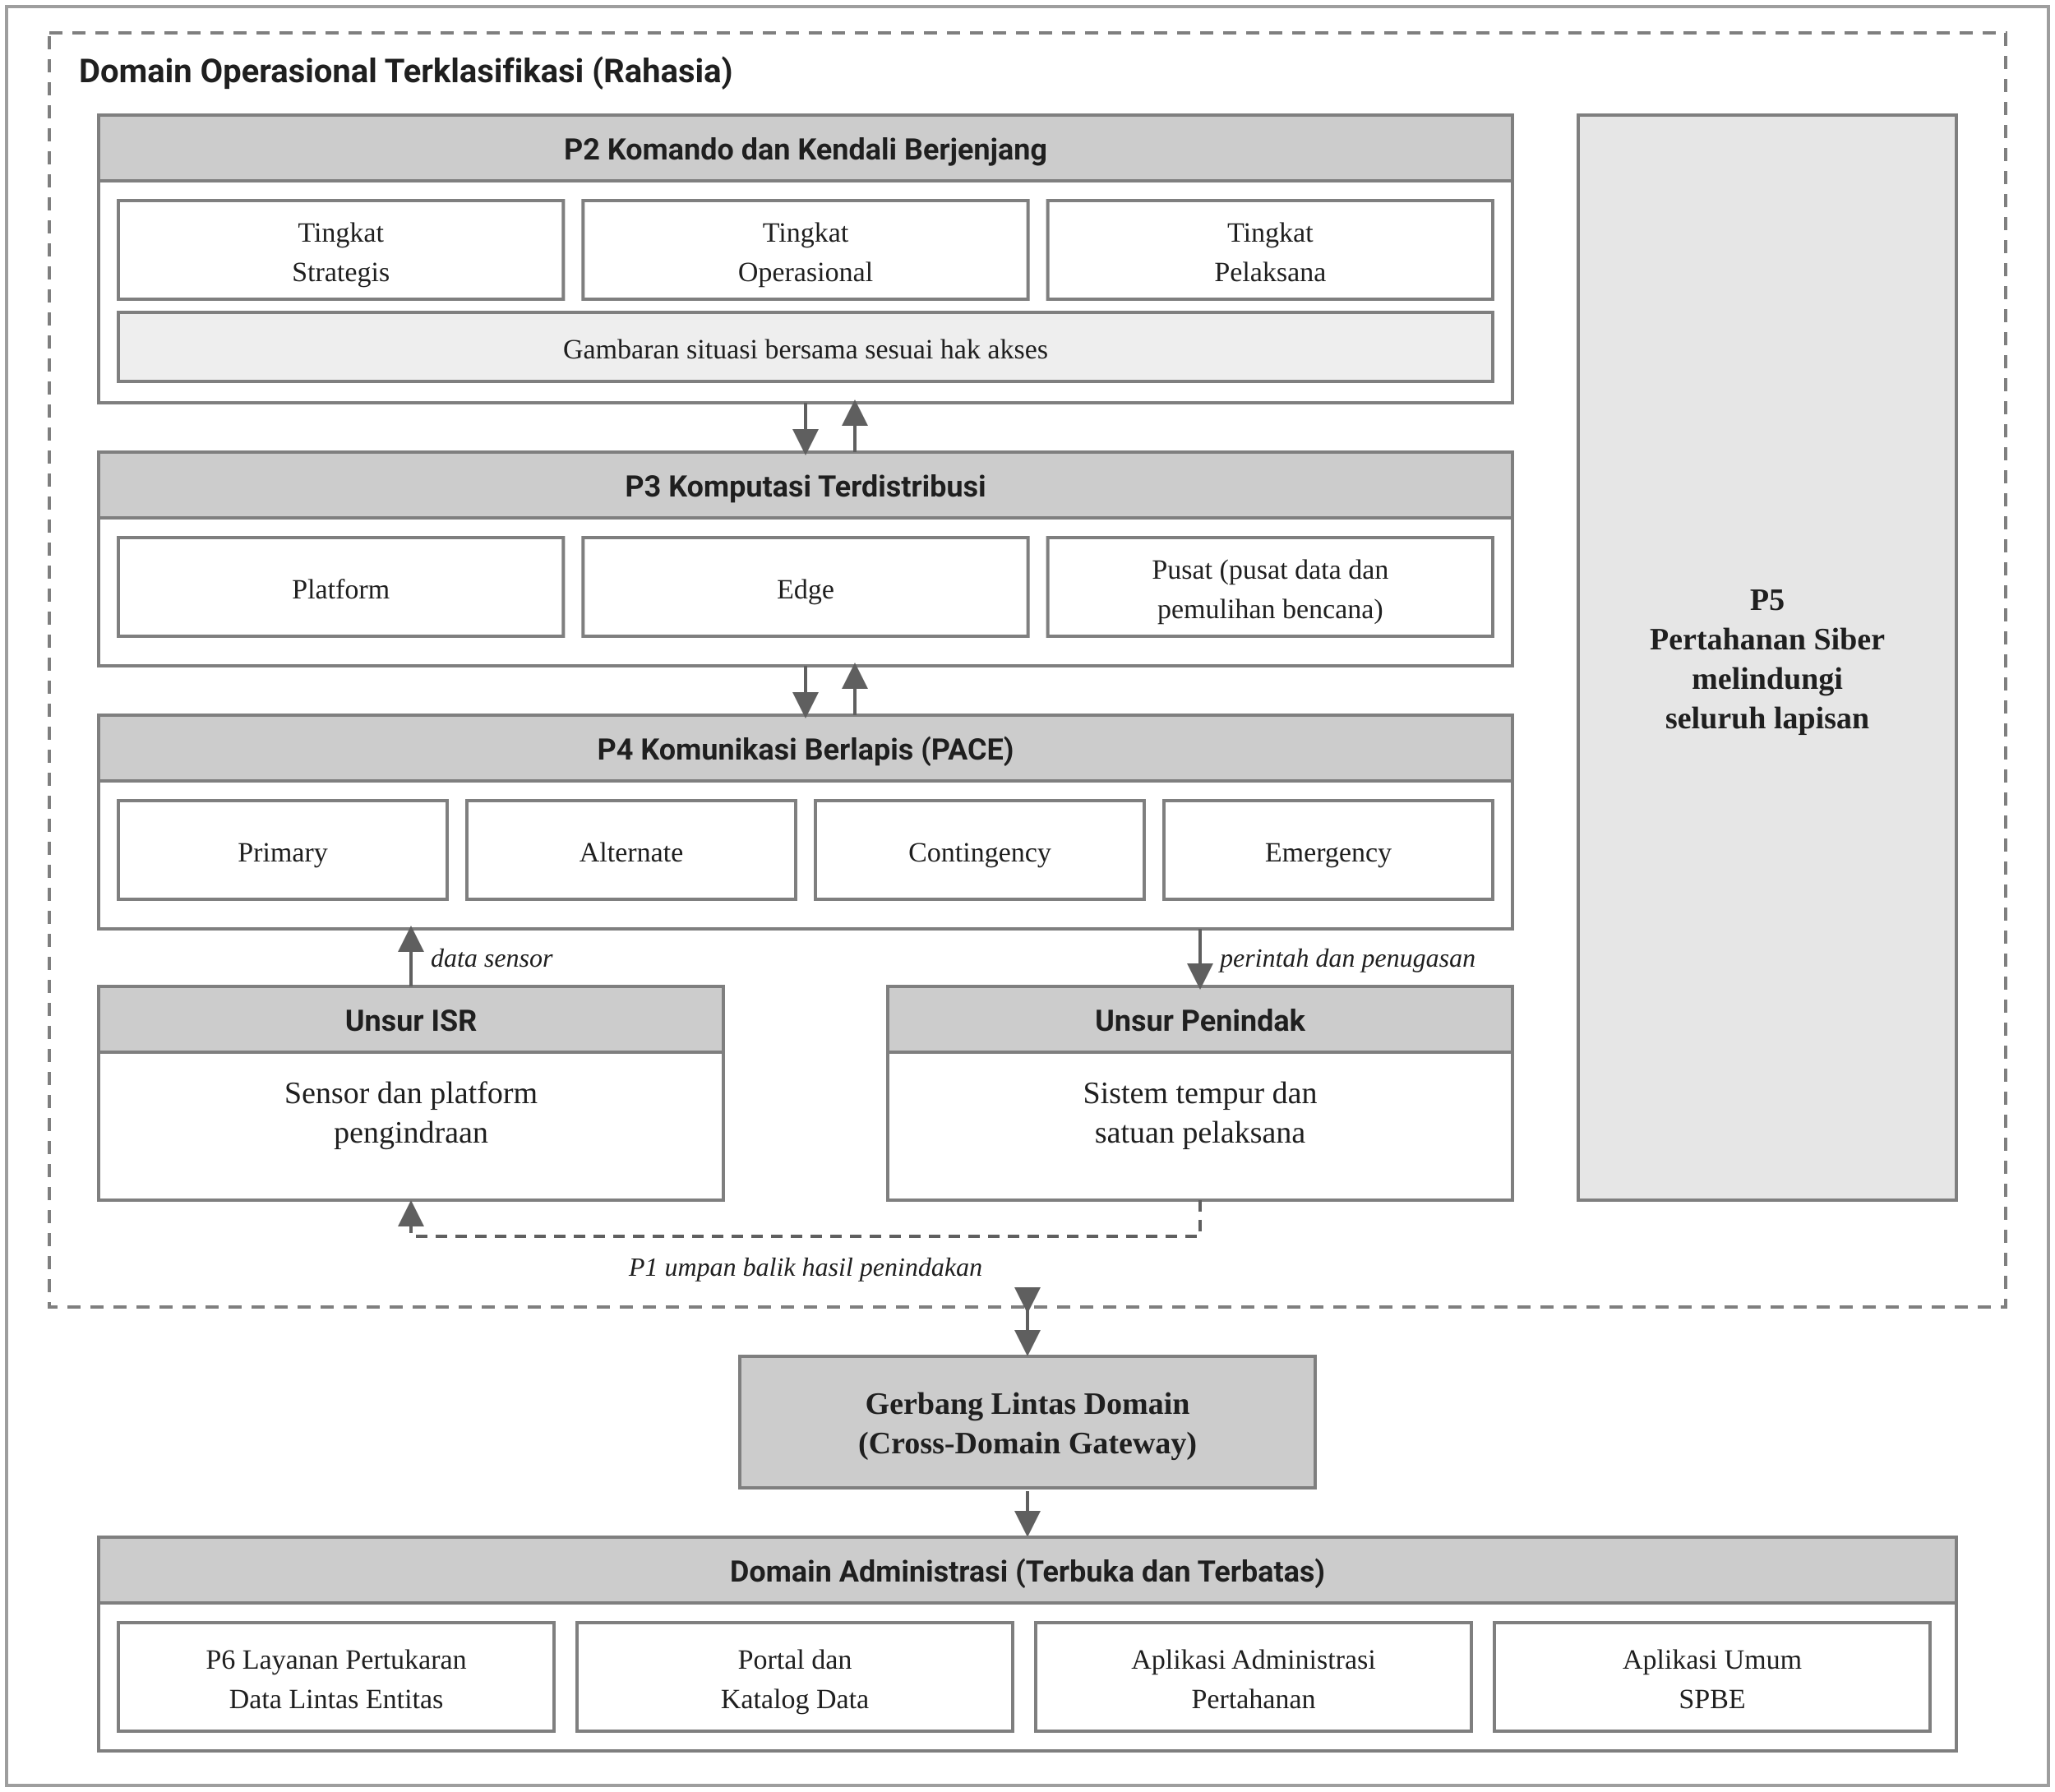
\includegraphics[width=1.00\linewidth,height=0.8\textheight,keepaspectratio]{images/Pola Arsitektur Lintas Domain C6ISR.png}
\caption{Pola Arsitektur Lintas Domain C6ISR}
\label{fig:III.4}
\end{figure}

Gambar~\ref{fig:III.4} menunjukkan bahwa seluruh unsur C6ISR berada pada domain operasional terklasifikasi, sedangkan pertukaran dengan domain administrasi dilakukan melalui gerbang lintas domain. Uraian setiap pola disajikan pada Tabel~\ref{tab:III.16}.

\begingroup\small\setstretch{1.0}
\begin{longtable}{@{}>{\raggedright\arraybackslash\hspace{0pt}}p{0.177\linewidth}>{\raggedright\arraybackslash\hspace{0pt}}p{0.238\linewidth}>{\raggedright\arraybackslash\hspace{0pt}}p{0.303\linewidth}>{\raggedright\arraybackslash\hspace{0pt}}p{0.189\linewidth}@{}}
\caption{Pola Arsitektur Lintas Domain C6ISR}\label{tab:III.16}\\
\toprule
\textbf{Pola} & \textbf{Masalah} & \textbf{Solusi Acuan} & \textbf{Unsur C6ISR}\\
\midrule
\endfirsthead
\multicolumn{4}{@{}l}{\small\itshape \tablename\ \thetable{} (lanjutan)}\\
\toprule
\textbf{Pola} & \textbf{Masalah} & \textbf{Solusi Acuan} & \textbf{Unsur C6ISR}\\
\midrule
\endhead
\bottomrule
\endlastfoot
P1 Siklus C6ISR tertutup & Data sensor, keputusan, dan penindakan terputus antarsistem. & Data ISR dialirkan melalui komunikasi dan komputasi ke komando-kendali, perintah diteruskan ke unsur penindak, dan hasilnya menjadi umpan balik. & Seluruh unsur\\*
P2 Komando dan kendali berjenjang & Setiap tingkat komando memiliki gambaran situasi yang berbeda. & Tingkat strategis, operasional, dan pelaksana menggunakan gambaran situasi yang sama sesuai hak aksesnya. & \textit{Command}, \textit{Control}\\
P3 Komputasi terdistribusi & Pengolahan terpusat gagal ketika koneksi terputus. & Komputasi pada tingkat platform, \textit{edge}, dan pusat yang dapat beroperasi mandiri dalam waktu terbatas. & \textit{Computers}\\
P4 Komunikasi berlapis & Gangguan pada satu media memutus komunikasi. & Skema PACE\label{sk:PACE}, yaitu jalur \textit{primary}, \textit{alternate}, \textit{contingency}, dan \textit{emergency} yang digunakan berurutan ketika jalur sebelumnya tidak tersedia \cite{CISAPACE2023}. & \textit{Communications}\\
P5 Pemisahan domain klasifikasi & Informasi Rahasia bercampur dengan informasi administrasi. & Jaringan operasional terklasifikasi terpisah, dengan pertukaran melalui gerbang lintas domain dan pertahanan siber pada seluruh lapisan. & \textit{Cyber-Defense}\\*
P6 Pertukaran data lintas entitas & Data terkotak per aplikasi dan per organisasi. & Layanan pertukaran data dengan kamus data bersama, portal dan katalog data, serta antarmuka standar. & \textit{Computers}, \textit{Communications}\\
\end{longtable}
\endgroup

Tabel~\ref{tab:III.16} menunjukkan bahwa setiap pola memadukan elemen lebih dari satu domain. Pola P1 menjadi pengikat utama keterpaduan C6ISR, sedangkan pola lainnya menjamin kondisi yang dibutuhkan P1, yaitu keputusan berjenjang, komputasi yang tangguh, komunikasi berlapis, keamanan, dan pertukaran data.

\subsection{Aspek Keamanan, Interoperabilitas, Tata Kelola, dan Kepatuhan}
\label{sec:III.4.7}

Aspek lintas domain berlaku pada seluruh komponen DERA, sebagaimana disajikan pada Tabel~\ref{tab:III.17}.

\begingroup\small\setstretch{1.0}
\begin{longtable}{@{}>{\raggedright\arraybackslash\hspace{0pt}}p{0.201\linewidth}>{\raggedright\arraybackslash\hspace{0pt}}p{0.524\linewidth}>{\raggedright\arraybackslash\hspace{0pt}}p{0.213\linewidth}@{}}
\caption{Aspek Lintas Domain DERA}\label{tab:III.17}\\
\toprule
\textbf{Aspek} & \textbf{Ketentuan Acuan} & \textbf{Dasar}\\
\midrule
\endfirsthead
\multicolumn{3}{@{}l}{\small\itshape \tablename\ \thetable{} (lanjutan)}\\
\toprule
\textbf{Aspek} & \textbf{Ketentuan Acuan} & \textbf{Dasar}\\
\midrule
\endhead
\bottomrule
\endlastfoot
Keamanan & Klasifikasi tiga tingkat, kendali keamanan per domain klasifikasi, sistem manajemen keamanan informasi, dan target kematangan keamanan siber sesuai peta jalan pelindungan infrastruktur informasi vital. & \cite{Permenhan1Tahun2023,Permenhan82Tahun2014,Permenhan34Tahun2025,ISO27001}\\*
Interoperabilitas & Kosakata bersama, kamus data bersama, standar pertukaran data, dan antarmuka terbuka antarorganisasi pertahanan. & \cite{Permenhan1Tahun2023,Perpres132Tahun2022}\\
Tata kelola & Pemilik DERA di tingkat kementerian, dewan arsitektur, pengelolaan versi DERA, dan tinjauan kesesuaian arsitektur turunan. & \cite{TOGAF2022}\\*
Kepatuhan & Keselarasan dengan Arsitektur SPBE, Satu Data Indonesia dan Satu Data Pertahanan, serta pelindungan infrastruktur informasi vital. & \cite{Perpres132Tahun2022,Perpres39Tahun2019,Permenhan1Tahun2023,Permenhan34Tahun2025}\\
\end{longtable}
\endgroup

Untuk memenuhi KR-06, setiap domain DERA juga dipetakan ke domain Arsitektur SPBE, sebagaimana disajikan pada Tabel~\ref{tab:III.18}.

\begingroup\small\setstretch{1.0}
\begin{longtable}{@{}>{\raggedright\arraybackslash\hspace{0pt}}p{0.403\linewidth}>{\raggedright\arraybackslash\hspace{0pt}}p{0.566\linewidth}@{}}
\caption{Pemetaan Komponen DERA dan Domain Arsitektur SPBE}\label{tab:III.18}\\
\toprule
\textbf{Komponen DERA} & \textbf{Domain Arsitektur SPBE}\\
\midrule
\endfirsthead
\multicolumn{2}{@{}l}{\small\itshape \tablename\ \thetable{} (lanjutan)}\\
\toprule
\textbf{Komponen DERA} & \textbf{Domain Arsitektur SPBE}\\
\midrule
\endhead
\bottomrule
\endlastfoot
\textit{Business Reference Architecture} & Proses Bisnis dan Layanan\\*
\textit{Data Reference Architecture} & Data dan Informasi\\
\textit{Application Reference Architecture} & Aplikasi\\
\textit{Technology Reference Architecture} & Infrastruktur\\
Aspek keamanan & Keamanan\\*
\textit{Capability Reference Model} dan pola lintas domain & Tidak memiliki padanan (muatan khas pertahanan)\\
\end{longtable}
\endgroup

Tabel~\ref{tab:III.18} menunjukkan bahwa keempat domain dan aspek keamanan DERA berpadanan dengan domain Arsitektur SPBE \cite{Perpres132Tahun2022}, sehingga arsitektur turunan dapat sekaligus memenuhi kewajiban Arsitektur SPBE. CRM dan pola lintas domain tidak memiliki padanan karena merupakan muatan khas pertahanan.

\subsection{Standar dan Building Blocks}
\label{sec:III.4.8}

Posisi teknis DERA menetapkan standar yang wajib diikuti arsitektur turunan, sebagaimana disajikan pada Tabel~\ref{tab:III.19}.

\begingroup\small\setstretch{1.0}
\begin{longtable}{@{}>{\raggedright\arraybackslash\hspace{0pt}}p{0.236\linewidth}>{\raggedright\arraybackslash\hspace{0pt}}p{0.441\linewidth}>{\raggedright\arraybackslash\hspace{0pt}}p{0.260\linewidth}@{}}
\caption{Posisi Teknis DERA}\label{tab:III.19}\\
\toprule
\textbf{Kategori} & \textbf{Ketentuan} & \textbf{Acuan}\\
\midrule
\endfirsthead
\multicolumn{3}{@{}l}{\small\itshape \tablename\ \thetable{} (lanjutan)}\\
\toprule
\textbf{Kategori} & \textbf{Ketentuan} & \textbf{Acuan}\\
\midrule
\endhead
\bottomrule
\endlastfoot
Arsitektur & Pengembangan dan pemodelan arsitektur turunan & TOGAF \cite{TOGAF2022}, ArchiMate \cite{ArchiMate2019}\\*
Data & Kamus data, metadata, dan klasifikasi data & Satu Data Indonesia \cite{Perpres39Tahun2019}, Satu Data Pertahanan \cite{Permenhan1Tahun2023}\\
Keamanan & Sistem manajemen keamanan informasi dan pertahanan siber & ISO/IEC 27001 \cite{ISO27001}, Pedoman Pertahanan Siber \cite{Permenhan82Tahun2014}\\
Pemerintahan digital & Keselarasan arsitektur dan aplikasi umum & Arsitektur SPBE Nasional \cite{Perpres132Tahun2022}\\*
Interoperabilitas pertahanan & Standar pertukaran data dan antarmuka yang ditetapkan bersama antarorganisasi pertahanan & NISP\label{sk:NISP} sebagai pembanding \cite{NATONISP}\\
\end{longtable}
\endgroup

Posisi teknis tersebut diwujudkan dalam \textit{Architecture Building Blocks} (ABB) yang dapat digunakan ulang oleh arsitektur turunan, sebagaimana disajikan pada Tabel~\ref{tab:III.20}.

\begingroup\small\setstretch{1.0}
\begin{longtable}{@{}>{\raggedright\arraybackslash\hspace{0pt}}p{0.099\linewidth}>{\raggedright\arraybackslash\hspace{0pt}}p{0.368\linewidth}>{\raggedright\arraybackslash\hspace{0pt}}p{0.144\linewidth}>{\raggedright\arraybackslash\hspace{0pt}}p{0.133\linewidth}>{\raggedright\arraybackslash\hspace{0pt}}p{0.133\linewidth}@{}}
\caption{Katalog \textit{Architecture Building Blocks} DERA}\label{tab:III.20}\\
\toprule
\textbf{Kode} & \textbf{\textit{Building Block}} & \textbf{Domain} & \textbf{Pola} & \textbf{KR}\\
\midrule
\endfirsthead
\multicolumn{5}{@{}l}{\small\itshape \tablename\ \thetable{} (lanjutan)}\\
\toprule
\textbf{Kode} & \textbf{\textit{Building Block}} & \textbf{Domain} & \textbf{Pola} & \textbf{KR}\\
\midrule
\endhead
\bottomrule
\endlastfoot
ABB-01 & Layanan identitas dan akses tunggal & Aplikasi & P5 & KR-03\\*
ABB-02 & Layanan pertukaran data lintas entitas & Aplikasi & P6 & KR-04\\
ABB-03 & Portal dan katalog data & Data & P6 & KR-06\\
ABB-04 & Gambaran situasi bersama & Aplikasi & P1, P2 & KR-01\\
ABB-05 & Fusi data multi-sensor & Aplikasi & P1 & KR-01\\
ABB-06 & Antarmuka komando-kendali dengan sistem tempur & Aplikasi & P1 & KR-01\\
ABB-07 & Analitik dan dukungan keputusan & Aplikasi & P1 & KR-01\\
ABB-08 & Pusat data dan pemulihan bencana aktif-aktif & Teknologi & P3 & KR-01\\
ABB-09 & \textit{Node} komputasi \textit{edge} & Teknologi & P3 & KR-01\\
ABB-10 & Komunikasi berlapis PACE & Teknologi & P4 & KR-01\\
ABB-11 & Jaringan operasional terklasifikasi dan gerbang lintas domain & Teknologi & P5 & KR-03\\*
ABB-12 & Pusat operasi keamanan & Teknologi & P5 & KR-03\\
\end{longtable}
\endgroup

Tabel~\ref{tab:III.20} menunjukkan bahwa setiap ABB terhubung dengan pola dan kebutuhan arsitektur referensi. Kedudukan ABB terhadap posisi teknis dan arsitektur turunan ditunjukkan pada Gambar~\ref{fig:III.5}.

\begin{figure}[htbp]
\centering
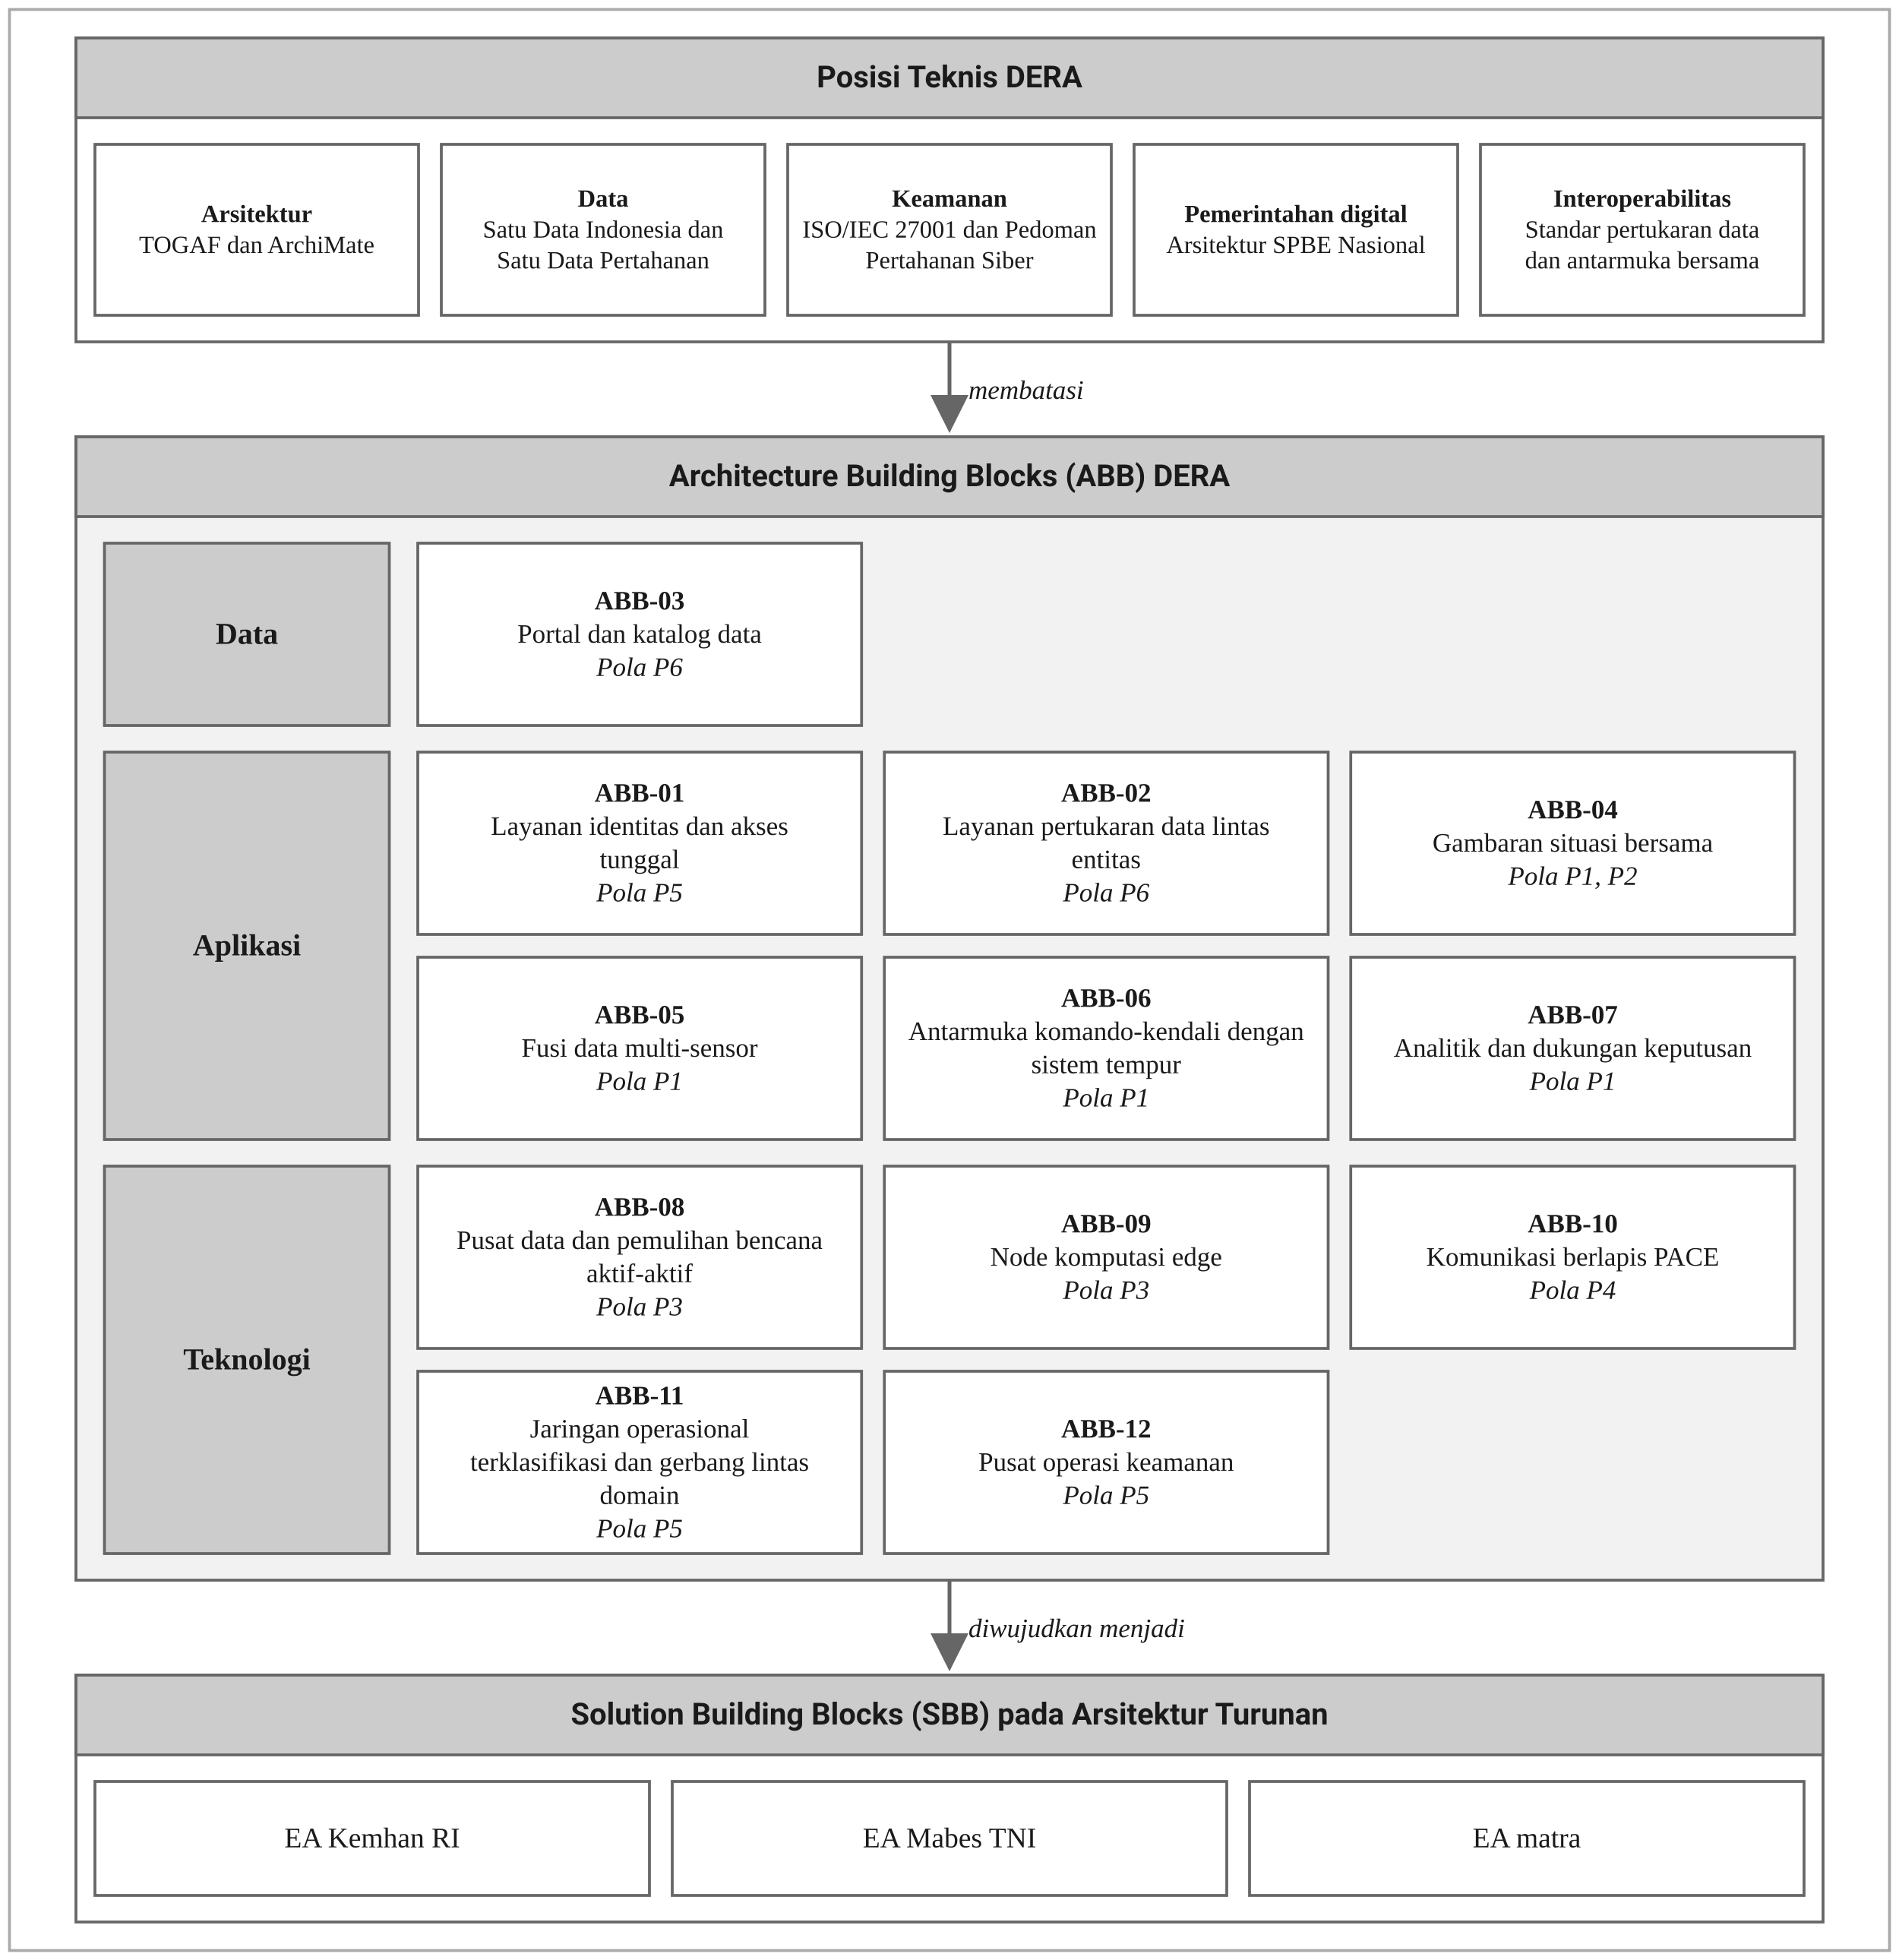
\includegraphics[width=1.00\linewidth,height=0.8\textheight,keepaspectratio]{images/Architecture Building Blocks DERA.png}
\caption{\textit{Architecture Building Blocks} DERA}
\label{fig:III.5}
\end{figure}

Gambar~\ref{fig:III.5} menunjukkan bahwa ABB DERA tersebar pada domain data, aplikasi, dan teknologi, dan setiap ABB menerapkan satu atau dua pola lintas domain. Posisi teknis membatasi spesifikasi setiap ABB, sedangkan arsitektur turunan, yaitu EA Kemhan RI, EA Mabes TNI, dan EA matra, mewujudkan ABB menjadi \textit{Solution Building Block} (SBB) sesuai kondisi organisasinya.

\section{Panduan Penerapan DERA}
\label{sec:III.5}

Panduan penerapan menjelaskan cara organisasi pertahanan menggunakan DERA untuk menyusun arsitektur turunan.

\subsection{Kedudukan DERA dalam Enterprise Continuum dan Architecture Repository}
\label{sec:III.5.1}

Dalam \textit{Enterprise Continuum}, DERA berada pada tingkat \textit{Industry Architecture}, yaitu arsitektur yang memuat komponen khusus suatu sektor \cite{TOGAF2022}. DERA diselaraskan dengan Arsitektur SPBE Nasional sebagai acuan arsitektur pemerintahan, dan mengarahkan arsitektur organisasi pertahanan pada tingkat \textit{Organization-Specific Architecture}, sebagaimana ditunjukkan pada Gambar~\ref{fig:III.6}.

\begin{figure}[htbp]
\centering
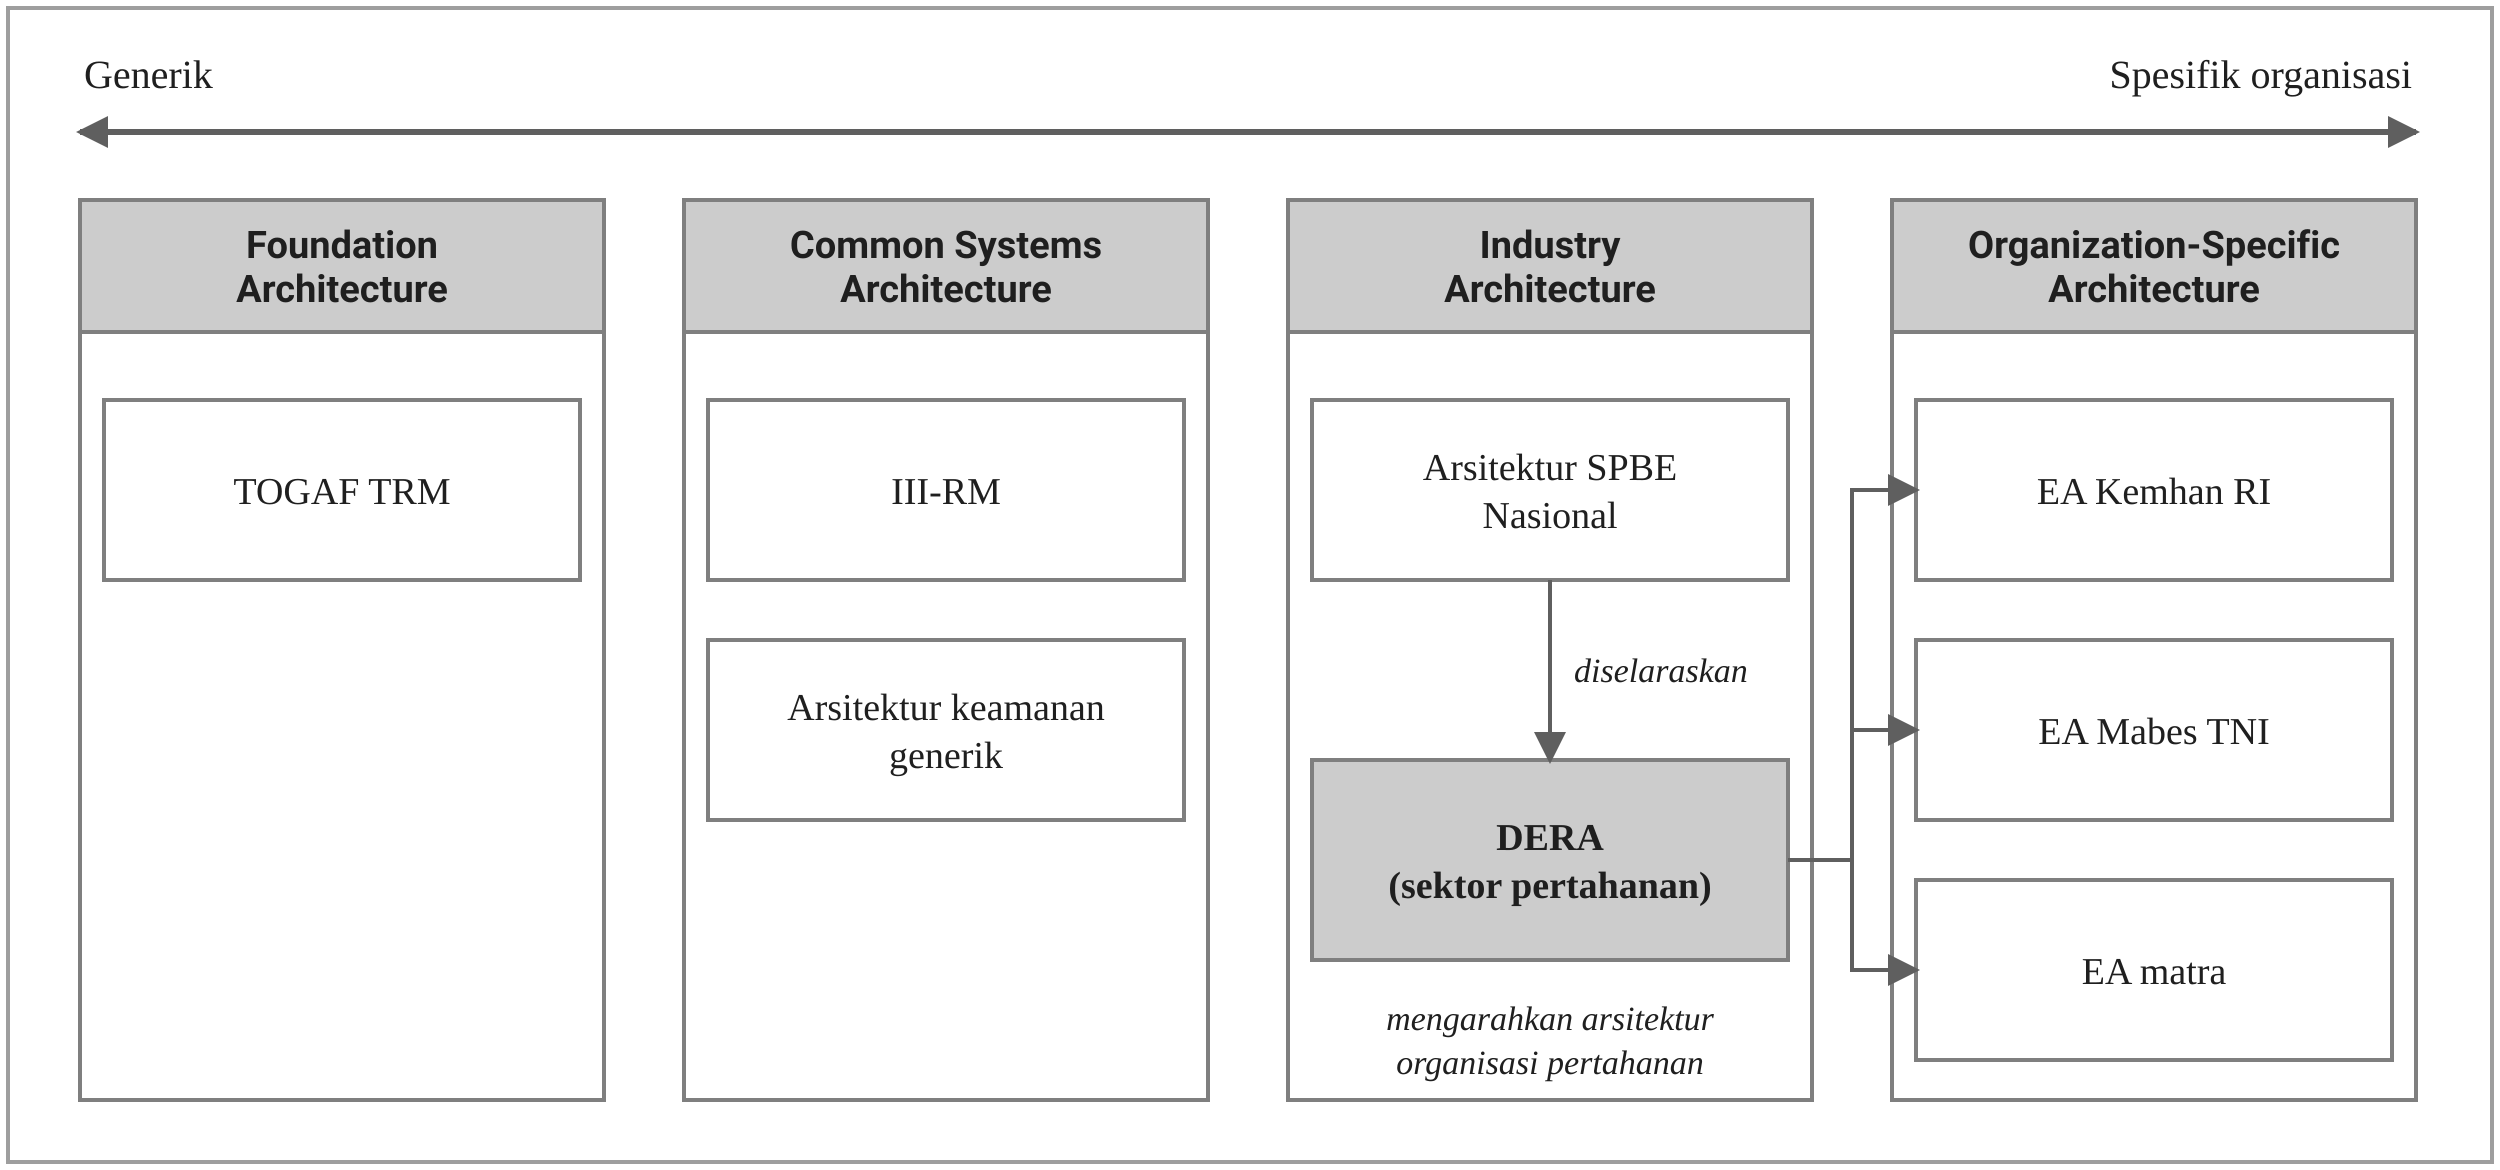
\includegraphics[width=1.00\linewidth,height=0.8\textheight,keepaspectratio]{images/Kedudukan DERA dalam Enterprise Continuum.png}
\caption{Kedudukan DERA dalam \textit{Enterprise Continuum}}
\label{fig:III.6}
\end{figure}

Gambar~\ref{fig:III.6} menunjukkan bahwa satu DERA dapat diturunkan menjadi beberapa arsitektur organisasi, yaitu EA Kemhan RI, EA Mabes TNI, dan EA matra. Dengan demikian, keterpaduan lintas organisasi pertahanan dibangun dari acuan yang sama. Di dalam \textit{Architecture Repository}, komponen DERA disimpan pada kelas yang sesuai, sebagaimana disajikan pada Tabel~\ref{tab:III.21}.

\begingroup\small\setstretch{1.0}
\begin{longtable}{@{}>{\raggedright\arraybackslash\hspace{0pt}}p{0.354\linewidth}>{\raggedright\arraybackslash\hspace{0pt}}p{0.615\linewidth}@{}}
\caption{Penempatan Komponen DERA dalam \textit{Architecture Repository}}\label{tab:III.21}\\
\toprule
\textbf{Kelas \textit{Architecture Repository}} & \textbf{Komponen DERA}\\
\midrule
\endfirsthead
\multicolumn{2}{@{}l}{\small\itshape \tablename\ \thetable{} (lanjutan)}\\
\toprule
\textbf{Kelas \textit{Architecture Repository}} & \textbf{Komponen DERA}\\
\midrule
\endhead
\bottomrule
\endlastfoot
\textit{Architecture Metamodel} & \textit{Metamodel} dan kosakata DERA\\*
\textit{Reference Library} & Tujuan strategis, prinsip, CRM, BRA, DRA, ARA, TRA, pola lintas domain, dan katalog ABB\\
\textit{Standards Library} & Posisi teknis DERA\\
\textit{Architecture Requirements Repository} & Kebutuhan arsitektur referensi (KR-01 hingga KR-10)\\
\textit{Governance Repository} & Kriteria kesesuaian, hasil tinjauan kesesuaian, dan catatan dispensasi\\*
\textit{Architecture Landscape} & Arsitektur turunan setiap organisasi pertahanan\\
\end{longtable}
\endgroup

Tabel~\ref{tab:III.21} menunjukkan bahwa sebagian besar komponen DERA berada pada \textit{Reference Library}, sedangkan posisi teknis berada pada \textit{Standards Library} karena bersifat wajib. Dengan penempatan tersebut, DERA dapat digunakan pada setiap fase ADM tanpa mengubah struktur TOGAF.

\subsection{Pemanfaatan DERA pada Fase ADM}
\label{sec:III.5.2}

DERA digunakan melalui siklus ADM baku tanpa fase tambahan. Titik masuk utamanya adalah langkah \textit{Select Reference Models, Viewpoints, and Tools} pada awal Fase B, C, dan D \cite{TOGAF2022}. Komponen DERA yang digunakan pada setiap fase ditunjukkan pada Gambar~\ref{fig:III.7}.

\begin{figure}[htbp]
\centering
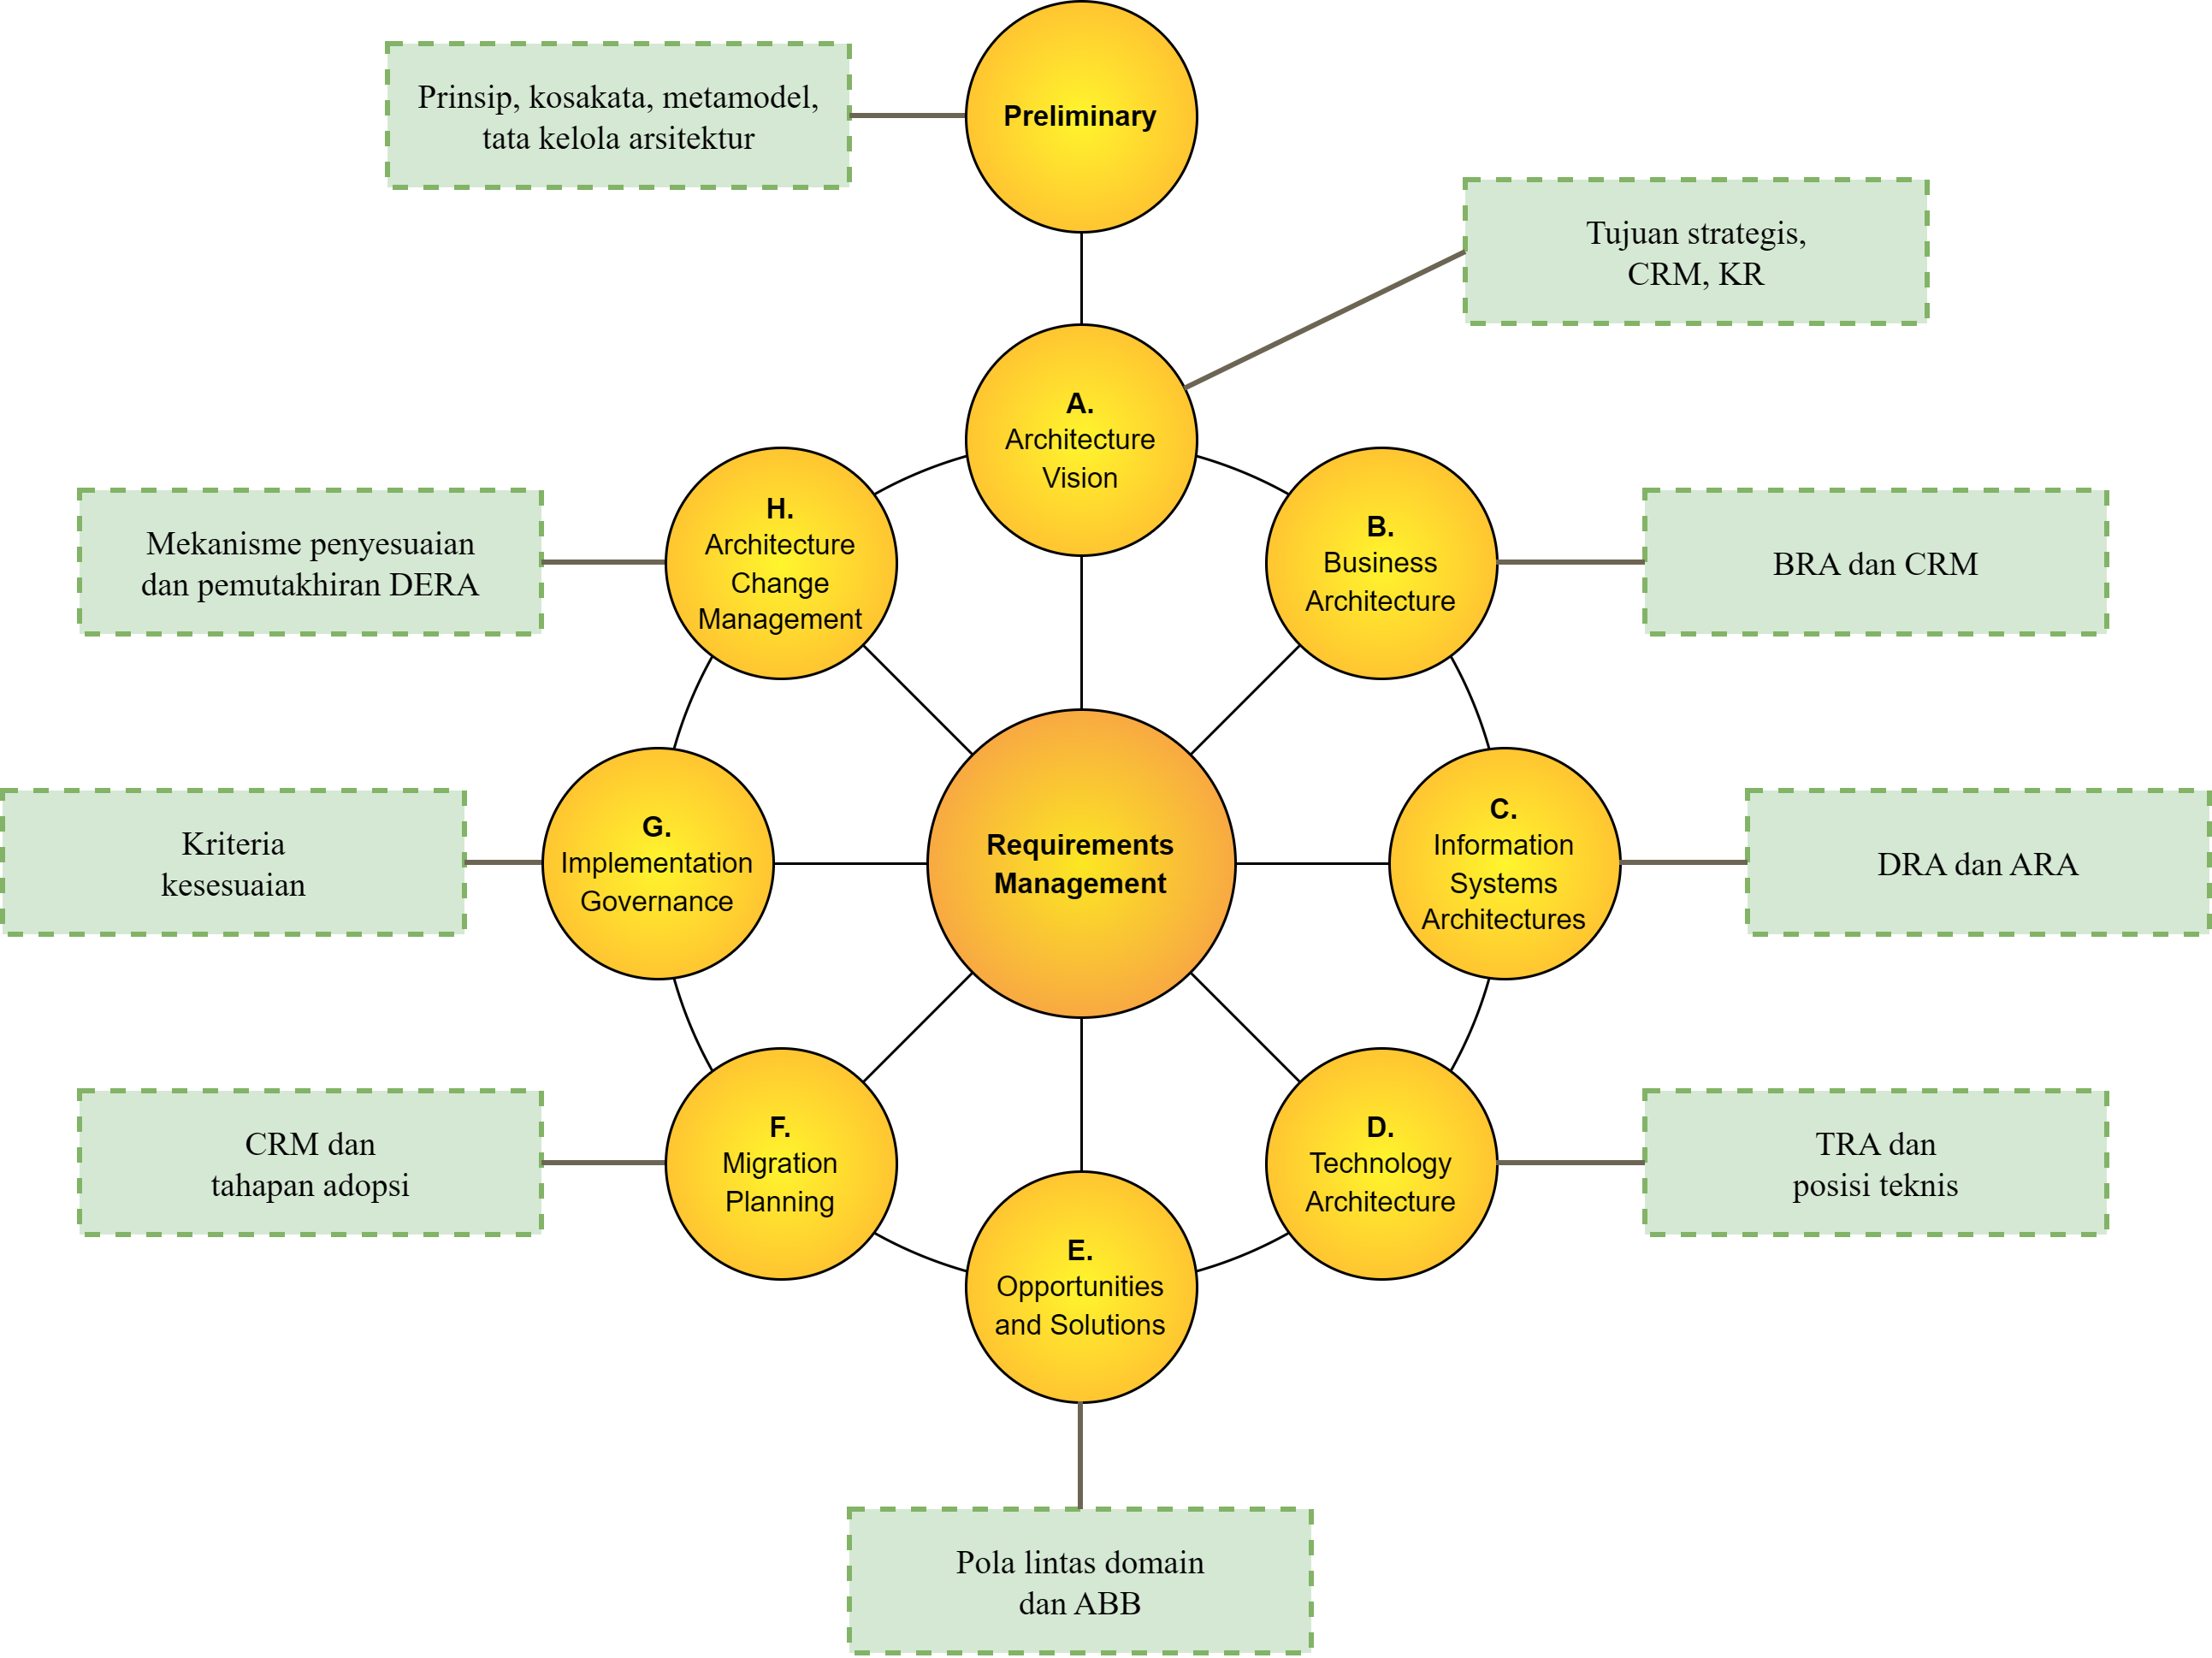
\includegraphics[width=0.94\linewidth,height=0.8\textheight,keepaspectratio]{images/TOGAF_ADM_Standar_dengan_Kotak_DERA.drawio.png}
\caption{Pemanfaatan DERA pada Siklus ADM}
\label{fig:III.7}
\end{figure}

Gambar~\ref{fig:III.7} menunjukkan bahwa setiap fase ADM memiliki komponen DERA sebagai masukannya. Cara pemanfaatan komponen tersebut disajikan pada Tabel~\ref{tab:III.22}.

\FloatBarrier % cegah longtable menabrak footer saat ada gambar tertunda
\begingroup\small\setstretch{1.0}
\begin{longtable}{@{}>{\raggedright\arraybackslash\hspace{0pt}}p{0.236\linewidth}>{\raggedright\arraybackslash\hspace{0pt}}p{0.236\linewidth}>{\raggedright\arraybackslash\hspace{0pt}}p{0.465\linewidth}@{}}
\caption{Pemanfaatan DERA pada Fase ADM}\label{tab:III.22}\\
\toprule
\textbf{Fase ADM} & \textbf{Komponen DERA} & \textbf{Pemanfaatan}\\
\midrule
\endfirsthead
\multicolumn{3}{@{}l}{\small\itshape \tablename\ \thetable{} (lanjutan)}\\
\toprule
\textbf{Fase ADM} & \textbf{Komponen DERA} & \textbf{Pemanfaatan}\\
\midrule
\endhead
\bottomrule
\endlastfoot
\textit{Preliminary} & Prinsip, kosakata, \textit{metamodel}, dan tata kelola arsitektur & Menetapkan DERA sebagai acuan, mengadopsi prinsip dan \textit{metamodel}, serta membentuk tata kelola arsitektur.\\*
A. \textit{Architecture Vision} & Tujuan strategis, CRM, dan KR & Menetapkan ruang lingkup berdasarkan lapis CRM yang sesuai mandat organisasi dan menautkan visi dengan sasaran strategis pertahanan.\\
B. \textit{Business Architecture} & BRA dan CRM & Menurunkan peta kapabilitas, aliran nilai, dan peran organisasi.\\
C. \textit{Information Systems Architectures} & DRA dan ARA & Menurunkan area subjek data, klasifikasi data, dan kategori aplikasi.\\
D. \textit{Technology Architecture} & TRA dan posisi teknis & Menurunkan layanan teknologi dan menerapkan standar wajib.\\
E. \textit{Opportunities and Solutions} & Pola lintas domain dan ABB & Mewujudkan ABB menjadi SBB dan menyusun paket solusi berdasarkan pola.\\
F. \textit{Migration Planning} & CRM dan tahapan adopsi & Menetapkan prioritas berdasarkan kapabilitas C6ISR yang paling dibutuhkan dan tahapan adopsi DERA.\\
G. \textit{Implementation Governance} & Kriteria kesesuaian & Melaksanakan \textit{Architecture Compliance Review} terhadap proyek dan arsitektur turunan.\\
H. \textit{Architecture Change Management} & Mekanisme penyesuaian & Mengelola perubahan arsitektur turunan dan mengusulkan pemutakhiran DERA.\\*
\textit{Requirements Management} & KR dan matriks keterlacakan & Mengelola kebutuhan dan menelusurinya ke komponen DERA.\\
\end{longtable}
\endgroup

Tabel~\ref{tab:III.22} menunjukkan bahwa DERA digunakan pada seluruh fase ADM. Selain itu, pola lintas domain digunakan sejak Fase B hingga D untuk menjaga keterpaduan siklus C6ISR, kemudian menjadi dasar paket solusi pada Fase E. Dengan demikian, keterpaduan C6ISR dicapai melalui model referensi dan pola yang digunakan pada fase ADM baku.

\subsection{Mekanisme Adopsi dan Penyesuaian}
\label{sec:III.5.3}

DERA disesuaikan melalui titik variasi, yaitu bagian yang dapat diubah tanpa melanggar inti arsitektur referensi \cite{Galster2011}. Tingkat keterikatan dan mekanisme penyesuaian setiap komponen disajikan pada Tabel~\ref{tab:III.23}.

\begingroup\small\setstretch{1.0}
\begin{longtable}{@{}>{\raggedright\arraybackslash\hspace{0pt}}p{0.272\linewidth}>{\raggedright\arraybackslash\hspace{0pt}}p{0.166\linewidth}>{\raggedright\arraybackslash\hspace{0pt}}p{0.501\linewidth}@{}}
\caption{Tingkat Keterikatan dan Mekanisme Penyesuaian Komponen DERA}\label{tab:III.23}\\
\toprule
\textbf{Komponen} & \textbf{Keterikatan} & \textbf{Mekanisme Penyesuaian}\\
\midrule
\endfirsthead
\multicolumn{3}{@{}l}{\small\itshape \tablename\ \thetable{} (lanjutan)}\\
\toprule
\textbf{Komponen} & \textbf{Keterikatan} & \textbf{Mekanisme Penyesuaian}\\
\midrule
\endhead
\bottomrule
\endlastfoot
Prinsip, kosakata, dan \textit{metamodel} & Wajib & Diadopsi utuh. Prinsip dapat ditambah sesuai mandat organisasi tanpa bertentangan dengan prinsip DERA.\\*
Posisi teknis dan pola P5 & Wajib & Diterapkan utuh. Penyimpangan hanya diperbolehkan melalui dispensasi yang tercatat.\\
CRM dan BRA & Disesuaikan & Seleksi lapis dan kapabilitas sesuai mandat, lalu spesialisasi menjadi kapabilitas yang lebih rinci.\\
DRA, ARA, dan TRA & Disesuaikan & Seleksi area dan kategori yang relevan, perluasan dengan elemen baru yang terlacak ke KR, serta penetapan klasifikasi akhir oleh pemilik data.\\*
Pola P1–P4, P6, dan ABB & Acuan & Diwujudkan menjadi SBB sesuai kondisi organisasi, teknologi, dan anggaran.\\
\end{longtable}
\endgroup

Tabel~\ref{tab:III.23} menunjukkan tiga tingkat keterikatan. Komponen wajib menjaga interoperabilitas dan keamanan lintas organisasi. Komponen yang disesuaikan memberi ruang bagi perbedaan mandat, misalnya Kemhan RI yang berfokus pada lapis strategis dan pengelolaan sumber daya, sedangkan matra berfokus pada lapis operasional. Komponen acuan memberi keleluasaan dalam memilih solusi.

Adopsi DERA dapat dilakukan bertahap sesuai kematangan arsitektur organisasi, sebagai berikut.

\begin{enumerate}[label=\arabic*.]
\item Tahap fondasi, yaitu mengadopsi prinsip, kosakata, \textit{metamodel}, dan tata kelola arsitektur.
\item Tahap domain, yaitu menurunkan arsitektur bisnis, data, aplikasi, dan teknologi dari model referensi DERA.
\item Tahap integrasi, yaitu menerapkan pola lintas domain dan ABB untuk mencapai keterpaduan siklus C6ISR.
\end{enumerate}

Pengalaman penerapan pada arsitektur turunan menjadi umpan balik bagi pemutakhiran DERA. Usulan perubahan dibahas oleh dewan arsitektur, kemudian ditetapkan sebagai versi baru DERA oleh pemilik DERA di tingkat kementerian. Mekanisme ini menjaga DERA tetap mutakhir terhadap perubahan regulasi, doktrin, dan teknologi.

\subsection{Kriteria Kesesuaian Arsitektur}
\label{sec:III.5.4}

Kriteria kesesuaian digunakan untuk menilai apakah arsitektur turunan telah mengikuti DERA, baik pada tinjauan kesesuaian di Fase G maupun pada demonstrasi di Bab IV. Kriteria tersebut disajikan pada Tabel~\ref{tab:III.24}.

\begingroup\small\setstretch{1.0}
\begin{longtable}{@{}>{\raggedright\arraybackslash\hspace{0pt}}p{0.103\linewidth}>{\raggedright\arraybackslash\hspace{0pt}}p{0.189\linewidth}>{\raggedright\arraybackslash\hspace{0pt}}p{0.467\linewidth}>{\raggedright\arraybackslash\hspace{0pt}}p{0.149\linewidth}@{}}
\caption{Kriteria Kesesuaian Arsitektur Turunan terhadap DERA}\label{tab:III.24}\\
\toprule
\textbf{Kode} & \textbf{Aspek} & \textbf{Kriteria} & \textbf{Sifat}\\
\midrule
\endfirsthead
\multicolumn{4}{@{}l}{\small\itshape \tablename\ \thetable{} (lanjutan)}\\
\toprule
\textbf{Kode} & \textbf{Aspek} & \textbf{Kriteria} & \textbf{Sifat}\\
\midrule
\endhead
\bottomrule
\endlastfoot
KK-01 & Prinsip & Arsitektur turunan mengadopsi seluruh prinsip DERA. & Wajib\\*
KK-02 & Kosakata dan \textit{metamodel} & Elemen dan hubungannya menggunakan istilah dan hubungan \textit{metamodel} DERA. & Wajib\\
KK-03 & Kapabilitas & Peta kapabilitas dipetakan ke CRM, dan unsur C6ISR yang relevan dengan mandat organisasi terwakili. & Wajib\\
KK-04 & Data & Setiap entitas data memiliki pemilik, klasifikasi tiga tingkat, dan definisi dalam kamus data. & Wajib\\
KK-05 & Aplikasi & Aplikasi dikelompokkan sesuai kategori ARA, aplikasi umum SPBE tidak dikembangkan ulang, dan pertukaran data dilakukan melalui layanan integrasi. & Wajib\\
KK-06 & Teknologi dan keamanan & Domain klasifikasi dipisahkan, dan pertukaran lintas domain dilakukan melalui gerbang lintas domain. & Wajib\\
KK-07 & Standar & Posisi teknis DERA diterapkan, atau penyimpangannya tercatat sebagai dispensasi. & Wajib\\
KK-08 & Solusi & ABB diwujudkan menjadi SBB dengan mengacu pada pola lintas domain. & Dianjurkan\\*
KK-09 & Keterlacakan & Setiap elemen arsitektur turunan dapat ditelusuri ke komponen DERA atau kebutuhan organisasi. & Wajib\\
\end{longtable}
\endgroup

Hasil pemeriksaan kriteria pada Tabel~\ref{tab:III.24} menentukan tingkat kesesuaian arsitektur turunan. Tingkat kesesuaian disederhanakan dari enam tingkat kesesuaian arsitektur pada TOGAF \cite{TOGAF2022} menjadi empat tingkat berikut.

\begin{enumerate}[label=\arabic*.]
\item Sesuai penuh, yaitu seluruh kriteria wajib dan anjuran terpenuhi.
\item Sesuai, yaitu seluruh kriteria wajib terpenuhi, dengan perluasan di luar DERA yang terlacak dan disetujui.
\item Konsisten, yaitu sebagian kriteria belum diterapkan, tetapi kriteria yang telah diterapkan sesuai dengan DERA. Tingkat ini merupakan kondisi wajar pada adopsi bertahap.
\item Tidak sesuai, yaitu terdapat elemen yang bertentangan dengan DERA tanpa dispensasi.
\end{enumerate}
